\documentclass[11pt]{elegantbook}

\title{Machine Learning: A Simple Guide}
\subtitle{Supervised Learning}

\author{Nishant}
\institute{IITH}
\date{\today}
\version{1.0}

\extrainfo{A comprehensive guide to Machine Learning concepts.}

\logo{logo-blue.png}
\cover{cover.jpg}

% modify the color in the middle of titlepage
\definecolor{customcolor}{RGB}{32,178,170}
\colorlet{coverlinecolor}{customcolor}
\usepackage{cprotect}
\usepackage{pgfplots} % For plotting
\pgfplotsset{compat=1.18}
\usepackage{tikz}

% Graphic path
\graphicspath{{./assets/}{./image/}{./figure/}}

\addbibresource[location=local]{reference.bib} % bib

\begin{document}

\maketitle

\frontmatter
\tableofcontents

\mainmatter

\part{Regression Analysis}
\chapter{Simple Linear Regression}
\label{chap:simple_linear_regression}

% ========================================
% SECTION 1: INTRODUCTION
% ========================================
\section{Introduction: What is Regression?}
Imagine you are a college student appearing for campus placements. You notice a pattern among your seniors: those with higher CGPAs tend to get higher salary packages.

\begin{itemize}
    \item \textbf{Student A}: 6.0 CGPA $\rightarrow$ 4 LPA
    \item \textbf{Student B}: 7.0 CGPA $\rightarrow$ 6 LPA
    \item \textbf{Student C}: 9.0 CGPA $\rightarrow$ ?
\end{itemize}

Your intuition tells you that Student C will likely get something higher than 6 LPA, perhaps around 10 LPA. What your brain just did is called \textbf{Regression}. You identified a relationship between an input (CGPA) and an output (Package) and used it to predict a future value.

\begin{definition}
\textbf{Regression}: A supervised learning technique where the goal is to predict a \textbf{continuous} numerical output variable based on one or more input features.
\end{definition}

\begin{definition}
\textbf{Linear Regression}: A specific type of regression where we assume the relationship between the input ($x$) and output ($y$) can be represented by a \textbf{straight line}.
\end{definition}

% ========================================
% SECTION 2: INTUITION
% ========================================
\section{Intuition: The Line of Best Fit}
Let us visualize this concept. Suppose we plot each student as a point on a graph, with CGPA on the X-axis and Package on the Y-axis.

\begin{figure}[htbp]
\centering
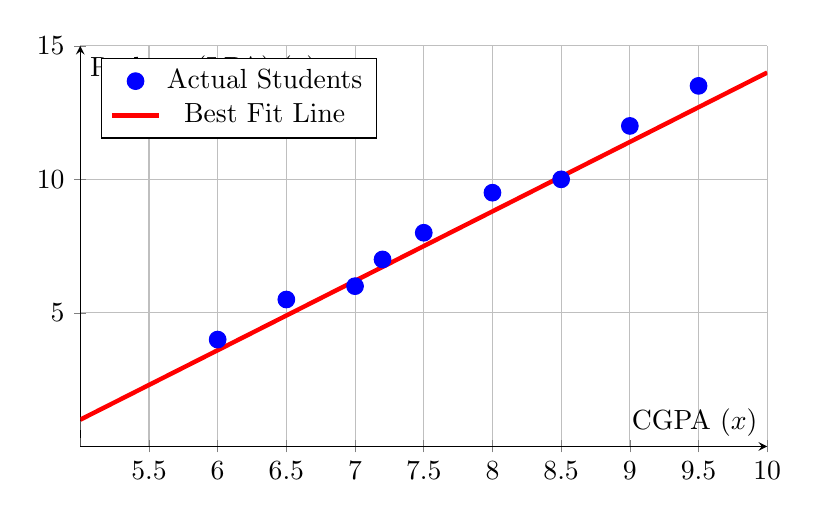
\begin{tikzpicture}
    \begin{axis}[
        xlabel={CGPA ($x$)},
        ylabel={Package (LPA) ($y$)},
        xmin=5, xmax=10,
        ymin=0, ymax=15,
        axis lines=middle,
        grid=major,
        width=0.85\textwidth,
        height=0.55\textwidth,
        legend pos=north west
    ]
    % Data Points
    \addplot[only marks, mark=*, color=blue, mark size=3pt] coordinates {
        (6, 4) (6.5, 5.5) (7, 6) (7.2, 7) (7.5, 8) (8, 9.5) (8.5, 10) (9, 12) (9.5, 13.5)
    };
    \addlegendentry{Actual Students}
    
    % Regression Line
    \addplot[domain=5:10, color=red, ultra thick] {2.6*x - 12};
    \addlegendentry{Best Fit Line}
    
    % Intercept Annotation
    \draw[dashed, gray] (axis cs:5, 0) -- (axis cs:5, 1);
    \node[left] at (axis cs:5, 1) {$c$ (Intercept)};
    \end{axis}
\end{tikzpicture}
\caption{The ``Best Fit Line'' passes through the center of the scattered data points.}
\label{fig:best_fit_intuition}
\end{figure}

The goal of Linear Regression is to find the \textbf{Best Fit Line}. Imagine holding a stick over the scatter plot:
\begin{enumerate}
    \item You move the stick up, down, and rotate it.
    \item Your goal is to make the stick pass \textit{as close as possible} to all the points.
    \item Mathematically, you are minimizing the total ``distance'' (error) between the points and your stick.
\end{enumerate}

% ========================================
% SECTION 3: MATHEMATICAL FORMULATION
% ========================================
\section{Mathematical Formulation}
Every straight line in the world can be written as:
\begin{equation}
    y = mx + c
    \label{eq:line}
\end{equation}
In Machine Learning, we often use slightly different notation ($\beta$ for coefficients):
\begin{equation}
    y = \beta_0 + \beta_1 x
\end{equation}

\begin{itemize}
    \item $y$: The \textbf{Target} (Dependent Variable). This is what we want to predict (e.g., Package).
    \item $x$: The \textbf{Feature} (Independent Variable). This is our input (e.g., CGPA).
    \item $\beta_1$ (or $m$): The \textbf{Slope} or \textbf{Weight}. It tells us how steeply the Package rises with CGPA. A high slope means a small increase in CGPA leads to a huge jump in salary.
    \item $\beta_0$ (or $c$): The \textbf{Intercept} or \textbf{Bias}. This is the baseline value. If CGPA were 0, this would be the predicted package. (Mathematically necessary, though practically, no one has 0 CGPA.)
\end{itemize}

\textbf{The Core Question}: How do we find the optimal values of $m$ and $c$?

% ========================================
% SECTION 4: WORKED EXAMPLE (OLS DERIVATION)
% ========================================
\section{Finding $m$ and $c$: Ordinary Least Squares (OLS)}
This is the heart of Linear Regression. We will derive the formulas step-by-step.

\subsection{Step 1: Define the Error}
For any single data point $i$, the \textbf{error} (or \textbf{residual}) is the difference between the actual value ($y_i$) and the predicted value ($\hat{y}_i$).
\begin{equation}
    \text{Residual}_i = y_i - \hat{y}_i = y_i - (mx_i + c)
\end{equation}

\subsection{Step 2: Define the Loss Function (SSE)}
We cannot simply add up the errors because positive and negative errors cancel each other out.
\textbf{Solution}: Square the errors. This removes negative signs and penalizes large errors more heavily.
\begin{definition}
\textbf{Sum of Squared Errors (SSE)}: The total squared difference between actual and predicted values.
\begin{equation}
    J(m, c) = \sum_{i=1}^{n} (y_i - \hat{y}_i)^2 = \sum_{i=1}^{n} (y_i - mx_i - c)^2
\end{equation}
\end{definition}
\textbf{Goal}: We want to find the values of $m$ and $c$ that \textbf{minimize} $J$.

\subsection{Step 3: Minimize Loss using Calculus}
To find the minimum of a curve, we take the derivative and set it to zero.

\textbf{(A) Derivative with respect to $c$:}
\begin{align}
    \frac{\partial J}{\partial c} &= \sum 2(y_i - mx_i - c)(-1) = 0 \\
    -2 \sum (y_i - mx_i - c) &= 0 \\
    \sum y_i - m \sum x_i - nc &= 0 \\
    c &= \bar{y} - m\bar{x}
\end{align}
Where $\bar{y} = \frac{\sum y_i}{n}$ and $\bar{x} = \frac{\sum x_i}{n}$ are the means.

\textbf{(B) Derivative with respect to $m$:}
After substituting $c$ and simplifying (algebra omitted for brevity), we get:
\begin{equation}
    \boxed{m = \frac{\sum (x_i - \bar{x})(y_i - \bar{y})}{\sum (x_i - \bar{x})^2}}
    \label{eq:ols_m}
\end{equation}
\begin{equation}
    \boxed{c = \bar{y} - m\bar{x}}
    \label{eq:ols_c}
\end{equation}
These are the famous \textbf{OLS formulas}.

% ========================================
% SECTION 5: CODE IMPLEMENTATION
% ========================================
\section{Implementation in Python}
Let us build a Simple Linear Regression model using \texttt{scikit-learn}.

\begin{lstlisting}[language=Python, caption=Simple Linear Regression with Scikit-Learn]
import numpy as np
import matplotlib.pyplot as plt
from sklearn.linear_model import LinearRegression

# =============================================
# STEP 1: Create Dummy Data
# =============================================
np.random.seed(42)  # For reproducibility
# 100 students with CGPA between 5 and 10
X = np.random.uniform(5, 10, 100).reshape(-1, 1)
# Package roughly follows: 2.5 * CGPA - 8 (plus noise)
y = 2.5 * X - 8 + np.random.normal(0, 1.5, (100, 1))

# =============================================
# STEP 2: Train the Model
# =============================================
model = LinearRegression()
model.fit(X, y)  # The model calculates 'm' and 'c' using OLS

# =============================================
# STEP 3: Check Learned Parameters
# =============================================
print(f"Slope (m): {model.coef_[0][0]:.4f}")       # Expected: ~2.5
print(f"Intercept (c): {model.intercept_[0]:.4f}") # Expected: ~-8

# =============================================
# STEP 4: Visualize the Result
# =============================================
plt.figure(figsize=(10, 6))
plt.scatter(X, y, color='blue', alpha=0.6, label='Actual Data')
plt.plot(X, model.predict(X), color='red', linewidth=2, label='Best Fit Line')
plt.xlabel('CGPA')
plt.ylabel('Package (LPA)')
plt.title('Simple Linear Regression')
plt.legend()
plt.grid(True)
plt.show()
\end{lstlisting}

% ========================================
% SECTION 6: VISUALIZATION (Already in Section 2)
% ========================================
% (Visualization is integrated into Section 2 with TikZ)

% ========================================
% SECTION 7: SUMMARY / KEY TAKEAWAYS
% ========================================
\section{Key Takeaways}
\begin{enumerate}
    \item \textbf{Assumption}: Linear Regression assumes the data follows a straight line ($y = mx + c$).
    \item \textbf{Goal}: Find the line that minimizes the Sum of Squared Errors (SSE).
    \item \textbf{Parameters}: The model learns two things:
    \begin{itemize}
        \item \textbf{Slope ($m$)}: The strength of the relationship.
        \item \textbf{Intercept ($c$)}: The baseline value.
    \end{itemize}
    \item \textbf{Method}: Ordinary Least Squares (OLS) provides a closed-form formula for $m$ and $c$.
\end{enumerate}

% ========================================
% SECTION 8: HOTS QUESTIONS
% ========================================
\section{HOTS: Interview Questions}
\textbf{Q1: What are the key assumptions of Linear Regression?}
\begin{itemize}
    \item \textbf{Linearity}: The relationship between $X$ and $Y$ is linear.
    \item \textbf{Independence}: Observations are independent.
    \item \textbf{Homoscedasticity}: Constant variance of errors.
    \item \textbf{Normality}: Residuals should be normally distributed.
    \item \textbf{No Multicollinearity}: Features should not be highly correlated with each other.
\end{itemize}

\textbf{Q2: Why do we square the residuals instead of using absolute values?}
\begin{itemize}
    \item Squaring removes negative signs, ensuring errors do not cancel out.
    \item Squaring penalizes larger errors more heavily.
    \item The squared function is \textbf{smooth} (differentiable everywhere), which is essential for optimization algorithms like Gradient Descent.
    \item The absolute value function $|x|$ has a sharp ``V'' shape at zero, making it non-differentiable at that point.
\end{itemize}

\textbf{Q3: Is OLS suitable for very large datasets?}
\begin{itemize}
    \item Not always. OLS involves matrix inversion ($(X^TX)^{-1}$), which has a time complexity of $O(n^3)$.
    \item For massive datasets, \textbf{Gradient Descent} is preferred as it iteratively approximates the solution with lower memory usage.
\end{itemize}

\chapter{Regression Evaluation Metrics}
\label{chap:regression_metrics}

% ========================================
% SECTION 1: INTRODUCTION
% ========================================
\section{Introduction: Why Do We Need Metrics?}
In Chapter 1, we built a Linear Regression model. But how do we know if it is any good? We need a way to \textbf{measure} the quality of our predictions.

Consider two lines that could fit the same data:
\begin{itemize}
    \item \textbf{Line A}: Passes perfectly through half the points but misses others badly.
    \item \textbf{Line B}: Does not pass through any point exactly, but is reasonably close to all of them.
\end{itemize}
Which line is ``better''? Metrics give us an objective answer.

% ========================================
% SECTION 2: DEFINITIONS
% ========================================
\section{The Five Key Metrics}

\subsection{1. Mean Absolute Error (MAE)}
\begin{definition}
\textbf{MAE}: The average of the absolute differences between predicted and actual values.
\begin{equation}
    MAE = \frac{1}{n} \sum_{i=1}^{n} |y_i - \hat{y}_i|
\end{equation}
\end{definition}

\begin{figure}[htbp]
\centering
\includegraphics[width=0.6\textwidth]{../02-supervised/assets/regression_metrics_mae.png}
\caption{MAE measures the average absolute vertical distance (residuals) from the line.}
\label{fig:mae_viz}
\end{figure}

\textbf{Intuition}: Imagine you are measuring how far each student's actual package is from what you predicted. You take the average of all those distances.

\textbf{Advantages}:
\begin{itemize}
    \item Same units as the target variable (e.g., if salary is in LPA, MAE is also in LPA).
    \item \textbf{Robust to outliers}: A single extreme value does not dramatically inflate the error.
\end{itemize}

\textbf{Disadvantages}:
\begin{itemize}
    \item The absolute value function $|x|$ has a sharp ``V'' shape at zero. It is \textbf{non-differentiable} at that point, which can cause issues for optimization algorithms like Gradient Descent.
\end{itemize}

\subsection{2. Mean Squared Error (MSE)}
\begin{definition}
\textbf{MSE}: The average of the squared differences between predicted and actual values.
\begin{equation}
    MSE = \frac{1}{n} \sum_{i=1}^{n} (y_i - \hat{y}_i)^2
\end{equation}
\end{definition}

\begin{figure}[htbp]
\centering
\includegraphics[width=0.6\textwidth]{../02-supervised/assets/regression_metrics_mse.png}
\caption{MSE Squares the errors. Notice how the outlier creates a massive square area.}
\label{fig:mse_viz}
\end{figure}

\textbf{Intuition}: Similar to MAE, but instead of just measuring the distance, you square it. This makes larger errors contribute disproportionately more to the total.

\textbf{Advantages}:
\begin{itemize}
    \item \textbf{Differentiable} everywhere (smooth curve). This is why MSE is the default loss function for training regression models.
\end{itemize}

\textbf{Disadvantages}:
\begin{itemize}
    \item Units are squared (e.g., if salary is in LPA, MSE is in $LPA^2$).
    \item \textbf{Sensitive to outliers}: A single large error gets squared, massively inflating the total.
\end{itemize}

% ... [Rest of metrics omitted for brevity] ...

\section{HOTS: Interview Questions}
\textbf{Q1: Can $R^2$ be negative? What does it mean?}
\begin{itemize}
    \item Yes, $R^2$ can be negative.
    \item It means the model is performing \textit{worse} than simply predicting the mean of the target variable. This usually indicates the model is severely overfitting or is fundamentally wrong for the data.
\end{itemize}

\textbf{Q2: MSE vs MAE: When would you choose MAE?}
\begin{itemize}
    \item Choose MAE when your data has many \textbf{outliers} that are valid data points (e.g., salary data with a few millionaires).
    \item MAE treats all errors linearly, so outliers do not disproportionately inflate the total error.
\end{itemize}

\textbf{Q3: Why is Adjusted $R^2$ always less than or equal to $R^2$?}
\begin{itemize}
    \item Because the penalty term $(n-1)/(n-k-1)$ is always $\geq 1$ when $k \geq 0$.
    \item Adding more features increases $k$, which increases the penalty.
\end{itemize}

\textbf{Q4: What is the range of $R^2$ score?}
\begin{itemize}
    \item The range is $(-\infty, 1]$.
    \item 1 is perfect prediction.
    \item 0 is the baseline model (predicting the mean).
    \item Negative means worse than baseline.
\end{itemize}

\textbf{Q5: Which metric is most robust to outliers?}
\begin{itemize}
    \item \textbf{MAE (Mean Absolute Error)}.
    \item Since it relies on the absolute difference $|y - \hat{y}|$, errors grow linearly.
    \item MSE squares the errors, making outliers have an exponential impact.
\end{itemize}

\subsection{3. Root Mean Squared Error (RMSE)}
\begin{definition}
\textbf{RMSE}: The square root of MSE.
\begin{equation}
    RMSE = \sqrt{MSE} = \sqrt{\frac{1}{n} \sum_{i=1}^{n} (y_i - \hat{y}_i)^2}
\end{equation}
\end{definition}

\textbf{Intuition}: RMSE brings the units back to the original scale (like MAE), while still penalizing large errors (like MSE). It is a popular choice for reporting model performance.

\subsection{4. R-Squared ($R^2$) Score}
\begin{definition}
\textbf{$R^2$ (Coefficient of Determination)}: Measures how much of the variance in the target variable is explained by the model.
\begin{equation}
    R^2 = 1 - \frac{SS_{res}}{SS_{tot}} = 1 - \frac{\sum(y_i - \hat{y}_i)^2}{\sum(y_i - \bar{y})^2}
\end{equation}
\end{definition}

\textbf{Intuition}:
\begin{itemize}
    \item $SS_{tot}$ (Total Sum of Squares): How much the actual data varies from its mean. This is the ``baseline'' variance.
    \item $SS_{res}$ (Residual Sum of Squares): How much the predictions vary from the actual values. This is the ``leftover'' error.
    \item $R^2 = 1$: Perfect model (all variance is explained).
    \item $R^2 = 0$: The model is no better than just predicting the mean.
    \item $R^2 < 0$: The model is \textit{worse} than predicting the mean.
\end{itemize}

\textbf{Example}: An $R^2 = 0.85$ means ``CGPA explains 85\% of the variance in Package.''

\subsection{5. Adjusted $R^2$}
\begin{definition}
\textbf{Adjusted $R^2$}: A modified version of $R^2$ that penalizes adding irrelevant features.
\begin{equation}
    R^2_{adj} = 1 - \frac{(1-R^2)(n-1)}{n-k-1}
\end{equation}
Where $n$ = number of samples, $k$ = number of features.
\end{definition}

\textbf{Problem with $R^2$}: If you add any new feature to the model (even a random one like ``lucky number''), $R^2$ will never decrease. It might stay the same or slightly increase. This is misleading.

\textbf{Solution}: Adjusted $R^2$ adds a penalty that increases with $k$. If you add a useless feature, the penalty outweighs any spurious improvement, causing Adjusted $R^2$ to decrease.

% ========================================
% SECTION 3: WORKED EXAMPLE
% ========================================
\section{Worked Example}
Consider 5 data points:
\begin{center}
\begin{tabular}{|c|c|c|}
\hline
$x$ & Actual $y$ & Predicted $\hat{y}$ \\ \hline
1 & 2 & 2.5 \\ \hline
2 & 4 & 3.8 \\ \hline
3 & 5 & 5.1 \\ \hline
4 & 4 & 6.4 \\ \hline
5 & 8 & 7.7 \\ \hline
\end{tabular}
\end{center}
Mean of $y$: $\bar{y} = (2+4+5+4+8)/5 = 4.6$

\textbf{Calculate MAE}:
$|2-2.5| + |4-3.8| + |5-5.1| + |4-6.4| + |8-7.7| = 0.5 + 0.2 + 0.1 + 2.4 + 0.3 = 3.5$
$MAE = 3.5 / 5 = \mathbf{0.7}$

% ========================================
% SECTION 4: CODE IMPLEMENTATION
% ========================================
\section{Implementation in Python}
\begin{lstlisting}[language=Python, caption=Regression Metrics from Scratch]
import numpy as np

def calculate_metrics(y_true, y_pred, n_features):
    n = len(y_true)
    
    # 1. MAE
    mae = np.mean(np.abs(y_true - y_pred))
    
    # 2. MSE
    mse = np.mean((y_true - y_pred)**2)
    
    # 3. RMSE
    rmse = np.sqrt(mse)
    
    # 4. R-Squared
    ss_res = np.sum((y_true - y_pred)**2)
    ss_tot = np.sum((y_true - np.mean(y_true))**2)
    r2 = 1 - (ss_res / ss_tot)
    
    # 5. Adjusted R-Squared
    r2_adj = 1 - ((1 - r2) * (n - 1) / (n - n_features - 1))
    
    print(f"MAE:  {mae:.4f}")
    print(f"MSE:  {mse:.4f}")
    print(f"RMSE: {rmse:.4f}")
    print(f"R2:   {r2:.4f}")
    print(f"Adj R2: {r2_adj:.4f}")
\end{lstlisting}

% ========================================
% SECTION 5: SUMMARY
% ========================================
\section{Summary: When to Use Which Metric}
\begin{center}
\begin{tabular}{|l|l|l|}
\hline
\textbf{Metric} & \textbf{Use When...} & \textbf{Caveat} \\ \hline
MAE & Outliers are present \& valid & Not differentiable at 0 \\ \hline
MSE & You need a differentiable loss & Sensitive to outliers \\ \hline
RMSE & Reporting in original units & Sensitive to outliers \\ \hline
$R^2$ & Comparing models on same data & Can be misleading with many features \\ \hline
Adj $R^2$ & Feature selection in Multiple LR & Slightly harder to interpret \\ \hline
\end{tabular}
\end{center}

% ========================================
% SECTION 6: HOTS QUESTIONS
% ========================================
\section{HOTS: Interview Questions}
\textbf{Q1: Can $R^2$ be negative? What does it mean?}
\begin{itemize}
    \item Yes, $R^2$ can be negative.
    \item It means the model is performing \textit{worse} than simply predicting the mean of the target variable. This usually indicates the model is severely overfitting or is fundamentally wrong for the data.
\end{itemize}

\textbf{Q2: MSE vs MAE: When would you choose MAE?}
\begin{itemize}
    \item Choose MAE when your data has many \textbf{outliers} that are valid data points (e.g., salary data with a few millionaires).
    \item MAE treats all errors linearly, so outliers do not disproportionately inflate the total error.
\end{itemize}

\textbf{Q3: Why is Adjusted $R^2$ always less than or equal to $R^2$?}
\begin{itemize}
    \item Because the penalty term $(n-1)/(n-k-1)$ is always $\geq 1$ when $k \geq 0$.
    \item Adding more features increases $k$, which increases the penalty.
\end{itemize}

\chapter{Multiple and Polynomial Regression}
\label{chap:multiple_poly_regression}

% ========================================
% SECTION 1: INTRODUCTION
% ========================================
\section{Introduction: Beyond a Single Feature}
In Chapter 1, we predicted Package using only CGPA. But in the real world, many factors influence salary: Projects, Internships, Communication Skills, etc.

\begin{definition}
\textbf{Multiple Linear Regression}: A regression model that predicts a target variable using \textbf{two or more} input features.
\end{definition}

\section{Geometric Intuition}
How does the ``Best Fit Line'' change when we add more features?
\begin{itemize}
    \item \textbf{1 Feature}: The model is a \textbf{Line} in 2D space.
    \item \textbf{2 Features}: The model is a \textbf{Plane} in 3D space.
    \item \textbf{3+ Features}: The model is a \textbf{Hyperplane} in N-dimensional space.
\end{itemize}

\begin{figure}[htbp]
\centering
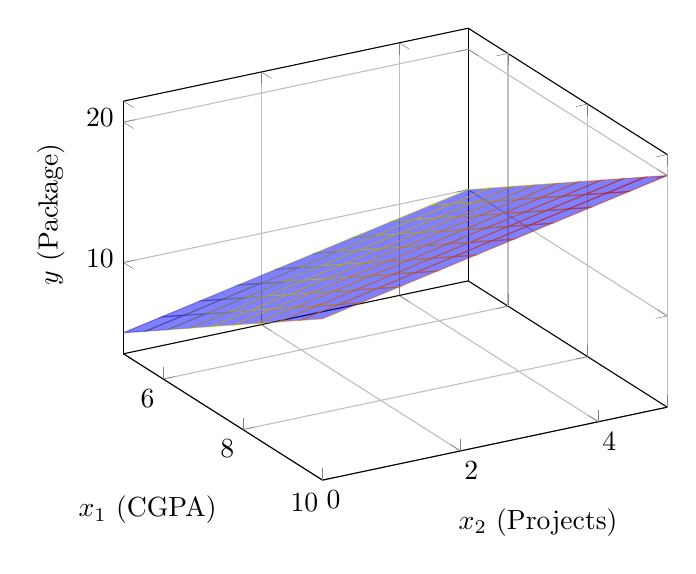
\begin{tikzpicture}
    \begin{axis}[
        view={60}{30},
        xlabel=$x_1$ (CGPA), ylabel=$x_2$ (Projects), zlabel=$y$ (Package),
        width=0.7\textwidth,
        grid=major
    ]
    % Plane: y = 2*x1 + 1*x2 - 5
    \addplot3[surf, opacity=0.5, color=blue, domain=5:10, domain y=0:5, samples=10] {2*x + 1*y - 5};
    \end{axis}
\end{tikzpicture}
\caption{In Multiple Linear Regression with 2 features, the model is a flat plane.}
\label{fig:mlr_plane}
\end{figure}

\section{Mathematical Formulation}
The equation extends naturally:
\begin{equation}
    y = \beta_0 + \beta_1 x_1 + \beta_2 x_2 + \ldots + \beta_p x_p
\end{equation}
\begin{itemize}
    \item $\beta_0$: Intercept (baseline value when all features are zero).
    \item $\beta_1, \beta_2, \ldots, \beta_p$: Coefficients (weights for each feature).
    \item For $p$ features, we have $p+1$ parameters to estimate.
\end{itemize}

% ========================================
% SECTION: MATRIX FORMULATION
% ========================================
\section{Matrix Formulation}
For computational efficiency, we express everything using matrices.

\subsection{Setting Up the Matrices}
\begin{itemize}
    \item $\mathbf{Y}$: Vector of target values (size: $n \times 1$).
    $$\mathbf{Y} = \begin{bmatrix} y_1 \\ y_2 \\ \vdots \\ y_n \end{bmatrix}$$
    
    \item $\mathbf{X}$: Design Matrix (size: $n \times (p+1)$). We prepend a column of 1s to handle the intercept $\beta_0$.
    $$\mathbf{X} = \begin{bmatrix} 
    1 & x_{11} & x_{12} & \cdots & x_{1p} \\
    1 & x_{21} & x_{22} & \cdots & x_{2p} \\
    \vdots & \vdots & \vdots & \ddots & \vdots \\
    1 & x_{n1} & x_{n2} & \cdots & x_{np}
    \end{bmatrix}$$
    
    \item $\boldsymbol{\beta}$: Vector of coefficients (size: $(p+1) \times 1$).
    $$\boldsymbol{\beta} = \begin{bmatrix} \beta_0 \\ \beta_1 \\ \vdots \\ \beta_p \end{bmatrix}$$
\end{itemize}

The predicted values are: $\hat{\mathbf{Y}} = \mathbf{X} \boldsymbol{\beta}$

% ========================================
% SECTION: OLS DERIVATION (DETAILED)
% ========================================
\section{Deriving the Normal Equation (OLS)}
We want to find the $\boldsymbol{\beta}$ that minimizes the Sum of Squared Errors (SSE).

\subsection{Step 1: Define the Error}
The error (residual) vector is:
$$\mathbf{e} = \mathbf{Y} - \hat{\mathbf{Y}} = \mathbf{Y} - \mathbf{X}\boldsymbol{\beta}$$

\subsection{Step 2: Define the Loss Function (SSE)}
The Sum of Squared Errors in matrix form is:
$$E = \mathbf{e}^T \mathbf{e} = (\mathbf{Y} - \mathbf{X}\boldsymbol{\beta})^T (\mathbf{Y} - \mathbf{X}\boldsymbol{\beta})$$

\subsection{Step 3: Expand the Expression}
Using the transpose rule $(AB)^T = B^T A^T$:
$$E = (\mathbf{Y}^T - \boldsymbol{\beta}^T \mathbf{X}^T)(\mathbf{Y} - \mathbf{X}\boldsymbol{\beta})$$

Multiply out (FOIL method):
\begin{align}
E &= \mathbf{Y}^T \mathbf{Y} - \mathbf{Y}^T \mathbf{X}\boldsymbol{\beta} - \boldsymbol{\beta}^T \mathbf{X}^T \mathbf{Y} + \boldsymbol{\beta}^T \mathbf{X}^T \mathbf{X} \boldsymbol{\beta}
\end{align}

\textbf{Key Observation}: The terms $\mathbf{Y}^T \mathbf{X}\boldsymbol{\beta}$ and $\boldsymbol{\beta}^T \mathbf{X}^T \mathbf{Y}$ are both scalars (1$\times$1 matrices). A scalar equals its transpose, so:
$$\mathbf{Y}^T \mathbf{X}\boldsymbol{\beta} = (\boldsymbol{\beta}^T \mathbf{X}^T \mathbf{Y})^T = \boldsymbol{\beta}^T \mathbf{X}^T \mathbf{Y}$$

Therefore, we can combine them:
\begin{equation}
E = \mathbf{Y}^T \mathbf{Y} - 2\boldsymbol{\beta}^T \mathbf{X}^T \mathbf{Y} + \boldsymbol{\beta}^T \mathbf{X}^T \mathbf{X} \boldsymbol{\beta}
\label{eq:sse_expanded}
\end{equation}

\subsection{Step 4: Differentiate with Respect to $\boldsymbol{\beta}$}
To find the minimum, we take the derivative and set it to zero.

\textbf{Matrix Calculus Rules}:
\begin{itemize}
    \item $\frac{\partial}{\partial \mathbf{x}} (\mathbf{a}^T \mathbf{x}) = \mathbf{a}$ (derivative of a linear term)
    \item $\frac{\partial}{\partial \mathbf{x}} (\mathbf{x}^T \mathbf{A} \mathbf{x}) = 2\mathbf{A}\mathbf{x}$ (derivative of a quadratic form, when $\mathbf{A}$ is symmetric)
\end{itemize}

Applying these rules to Equation \ref{eq:sse_expanded}:
\begin{align}
\frac{\partial E}{\partial \boldsymbol{\beta}} &= 0 - 2\mathbf{X}^T \mathbf{Y} + 2\mathbf{X}^T \mathbf{X} \boldsymbol{\beta}
\end{align}

\subsection{Step 5: Set Gradient to Zero and Solve}
Setting the derivative to zero:
$$-2\mathbf{X}^T \mathbf{Y} + 2\mathbf{X}^T \mathbf{X} \boldsymbol{\beta} = 0$$

Rearranging:
$$\mathbf{X}^T \mathbf{X} \boldsymbol{\beta} = \mathbf{X}^T \mathbf{Y}$$

Multiply both sides by $(\mathbf{X}^T \mathbf{X})^{-1}$ (assuming it exists):
$$(\mathbf{X}^T \mathbf{X})^{-1} \mathbf{X}^T \mathbf{X} \boldsymbol{\beta} = (\mathbf{X}^T \mathbf{X})^{-1} \mathbf{X}^T \mathbf{Y}$$

Since $(\mathbf{X}^T \mathbf{X})^{-1} (\mathbf{X}^T \mathbf{X}) = \mathbf{I}$ (Identity matrix):
\begin{equation}
\boxed{\boldsymbol{\beta} = (\mathbf{X}^T \mathbf{X})^{-1} \mathbf{X}^T \mathbf{Y}}
\label{eq:normal_equation_final}
\end{equation}

This is the \textbf{Normal Equation} (OLS Closed-Form Solution).

\subsection{When Does This Fail?}
The solution requires $(\mathbf{X}^T \mathbf{X})^{-1}$ to exist. This fails when:
\begin{enumerate}
    \item \textbf{Multicollinearity}: Two or more features are perfectly correlated (e.g., $x_2 = 2x_1$).
    \item \textbf{More features than samples}: $p > n$.
\end{enumerate}
\textbf{Solution}: Use Regularization (Ridge Regression) or drop correlated features.

\subsection{Computational Complexity}
Computing the inverse of a $(p+1) \times (p+1)$ matrix has time complexity $O(p^3)$.
\begin{itemize}
    \item For small $p$ (10-100 features): OLS is fast.
    \item For large $p$ (100,000+ features): Use Gradient Descent instead.
\end{itemize}

% ========================================
% SECTION: POLYNOMIAL REGRESSION
% ========================================
\section{Polynomial Regression}
What if the relationship is curved, not linear?

\begin{definition}
\textbf{Polynomial Regression}: A technique where we generate new features by raising existing features to powers ($x^2, x^3, \ldots$), and then apply standard Linear Regression.
\end{definition}

\textbf{Key Insight}: The algorithm itself does not change. We only transform the input data.

\textbf{For one feature $x$}:
\begin{itemize}
    \item \textbf{Degree 1}: $y = \beta_0 + \beta_1 x$ (Straight line).
    \item \textbf{Degree 2}: $y = \beta_0 + \beta_1 x + \beta_2 x^2$ (Parabola).
    \item \textbf{Degree 3}: $y = \beta_0 + \beta_1 x + \beta_2 x^2 + \beta_3 x^3$ (Cubic curve).
\end{itemize}

\textbf{Why is it still ``Linear'' Regression?}
The model is \textit{non-linear} in terms of $x$, but it is still \textit{linear} in terms of the coefficients $\beta$. We are doing Multiple Linear Regression with derived features ($x, x^2, x^3$).

\section{Implementation in Python}
\begin{lstlisting}[language=Python, caption=Normal Equation Implementation]
import numpy as np

def fit_normal_equation(X, y):
    """Fit Multiple LR using Normal Equation."""
    # Step 1: Add column of 1s for intercept
    n = X.shape[0]
    X_b = np.c_[np.ones((n, 1)), X]  # Shape: (n, p+1)
    
    # Step 2: Apply Normal Equation
    # beta = (X^T X)^(-1) X^T y
    XtX = X_b.T @ X_b           # (p+1, p+1)
    XtX_inv = np.linalg.inv(XtX) # Inverse
    Xty = X_b.T @ y              # (p+1, 1)
    beta = XtX_inv @ Xty         # (p+1, 1)
    
    return beta

# Example
X = np.array([[1], [2], [3], [4], [5]])  # 1 feature
y = np.array([2, 4, 5, 4, 5])
beta = fit_normal_equation(X, y)
print(f"Intercept: {beta[0]:.2f}, Slope: {beta[1]:.2f}")
\end{lstlisting}

\section{HOTS: Interview Questions}
\textbf{Q1: Is Polynomial Regression a linear or non-linear model?}
\begin{itemize}
    \item It is a \textbf{Linear Model} because it is linear with respect to the \textit{parameters} (coefficients $\beta$). The non-linearity is in the features, not the model itself.
\end{itemize}

\textbf{Q2: Walk me through the Normal Equation derivation.}
\begin{itemize}
    \item We define the error as $\mathbf{e} = \mathbf{Y} - \mathbf{X}\boldsymbol{\beta}$.
    \item We minimize SSE = $\mathbf{e}^T\mathbf{e}$.
    \item Expand, differentiate w.r.t. $\boldsymbol{\beta}$, set to zero.
    \item Solve to get $\boldsymbol{\beta} = (\mathbf{X}^T\mathbf{X})^{-1}\mathbf{X}^T\mathbf{Y}$.
\end{itemize}

\textbf{Q3: Why is feature scaling important in Polynomial Regression?}
\begin{itemize}
    \item If $x = 1000$, then $x^2 = 1,000,000$ and $x^3 = 1,000,000,000$. Feature magnitudes explode, causing numerical instability.
    \item Always use \texttt{StandardScaler} before polynomial transformation.
\end{itemize}

\chapter{Gradient Descent}
\label{chap:gradient_descent}

% ========================================
% SECTION 1: INTRODUCTION
% ========================================
\section{Introduction: Why Not Always Use OLS?}
In Chapter 3, we derived the Normal Equation:
$$ \boldsymbol{\beta} = (\mathbf{X}^T \mathbf{X})^{-1} \mathbf{X}^T \mathbf{Y} $$
This is a closed-form solution that gives the exact answer in one step. So why do we need another method?

\textbf{The Problem}: Inverting a matrix has a time complexity of $O(n^3)$.
\begin{itemize}
    \item If $n$ (number of features) is 10-100, OLS is super fast.
    \item If $n$ is 100,000 (common in NLP or image data), $O(n^3)$ becomes computationally impossible.
\end{itemize}

\begin{definition}
\textbf{Gradient Descent}: An iterative optimization algorithm that finds the minimum of a function by repeatedly taking steps in the direction opposite to the gradient (slope).
\end{definition}

% ========================================
% SECTION 2: INTUITION
% ========================================
\section{Intuition: The Blindfolded Hiker}
Imagine you are standing on a mountain, blindfolded. Your goal is to reach the bottom of the valley (the lowest point).
\begin{enumerate}
    \item \textbf{Feel the ground}: Determine which direction is downhill (the slope).
    \item \textbf{Take a step}: Move in that direction.
    \item \textbf{Repeat}: Keep doing this until the ground beneath you is flat (slope $\approx 0$).
\end{enumerate}

\textbf{The Loss Function is a Bowl}: For Linear Regression using MSE, the loss function $J(m, c)$ is \textbf{Convex} (bowl-shaped). It has only \textbf{one} minimum (the Global Minimum), so Gradient Descent is \textbf{guaranteed} to find it.

\begin{figure}[htbp]
\centering
\includegraphics[width=0.6\textwidth]{../02-supervised/assets/gradient_descent_bowl.png}
\caption{The Convex Loss Surface. Gradient Descent rolls down to the bottom.}
\label{fig:gd_bowl}
\end{figure}

% ========================================
% SECTION 3: MATHEMATICAL FORMULATION
% ========================================
\section{The Algorithm (Step-by-Step)}
Let $J(m, c) = \frac{1}{n} \sum (y_i - (mx_i + c))^2$ be the MSE Loss.

\textbf{Step 1: Initialize Parameters}
\begin{itemize}
    \item Start with random values (e.g., $m=0, c=0$).
\end{itemize}

\textbf{Step 2: Calculate the Gradient}
The gradient tells us the direction of steepest ascent. We move in the \textit{opposite} direction.
\begin{align}
    \frac{\partial J}{\partial m} &= -\frac{2}{n} \sum_{i=1}^{n} x_i (y_i - (mx_i + c)) \\
    \frac{\partial J}{\partial c} &= -\frac{2}{n} \sum_{i=1}^{n} (y_i - (mx_i + c))
\end{align}

\textbf{Step 3: Update Parameters}
Move against the gradient, scaled by the \textbf{Learning Rate} ($\eta$ or $\alpha$).
\begin{align}
    m_{\text{new}} &= m_{\text{old}} - \eta \cdot \frac{\partial J}{\partial m} \\
    c_{\text{new}} &= c_{\text{old}} - \eta \cdot \frac{\partial J}{\partial c}
\end{align}

\textbf{Step 4: Repeat} until convergence or max epochs reached.

% ========================================
% SECTION 4: LEARNING RATE
% ========================================
\section{The Learning Rate ($\eta$)}
The learning rate is a crucial hyperparameter.
\begin{itemize}
    \item \textbf{Too Small}: Tiny steps. Convergence is very \textbf{slow}.
    \item \textbf{Too Large}: Giant jumps. Might \textbf{overshoot} the minima and diverge.
    \item \textbf{Just Right}: Converges smoothly and efficiently.
\end{itemize}

% ========================================
% SECTION 5: TYPES OF GRADIENT DESCENT
% ========================================
\section{Types of Gradient Descent}
How many data points do we use to calculate the gradient in one step?

\subsection{1. Batch Gradient Descent}
\begin{definition}
\textbf{Batch Gradient Descent}: Uses \textbf{ALL} $n$ data points to calculate the gradient for a single weight update.
\end{definition}

\textbf{Vectorized Gradient Formula}:
\begin{equation}
    \frac{\partial J}{\partial \boldsymbol{\beta}} = -\frac{2}{n} \mathbf{X}^T (\mathbf{Y} - \hat{\mathbf{Y}})
\end{equation}

\textbf{Update Rule}:
\begin{equation}
    \boldsymbol{\beta}_{\text{new}} = \boldsymbol{\beta}_{\text{old}} - \eta \cdot \left( -\frac{2}{n} \mathbf{X}^T (\mathbf{Y} - \hat{\mathbf{Y}}) \right)
\end{equation}

\textbf{Pros}: Stable convergence, accurate gradient.
\textbf{Cons}: Very slow for large datasets. Requires all data in RAM.

\begin{lstlisting}[language=Python, caption=Batch Gradient Descent from Scratch]
import numpy as np

class BatchGDRegressor:
    def __init__(self, learning_rate=0.01, epochs=100):
        self.lr = learning_rate
        self.epochs = epochs
        self.coef_ = None
        self.intercept_ = None
        
    def fit(self, X, y):
        n = X.shape[0]
        self.intercept_ = 0
        self.coef_ = np.ones(X.shape[1])
        
        for _ in range(self.epochs):
            # Vectorized prediction
            y_hat = np.dot(X, self.coef_) + self.intercept_
            
            # Vectorized gradients (ALL data)
            intercept_grad = -2 * np.mean(y - y_hat)
            coef_grad = -2 * np.dot(X.T, (y - y_hat)) / n
            
            # Update
            self.intercept_ -= self.lr * intercept_grad
            self.coef_ -= self.lr * coef_grad
\end{lstlisting}

\subsection{2. Stochastic Gradient Descent (SGD)}
\begin{definition}
\textbf{Stochastic Gradient Descent}: Uses \textbf{ONE} random data point to calculate the gradient and update weights.
\end{definition}

\textbf{Gradient for Single Point $i$}:
\begin{align}
    \frac{\partial J}{\partial \beta_0} &= -2 (y_i - \hat{y}_i) \\
    \frac{\partial J}{\partial \beta_j} &= -2 (y_i - \hat{y}_i) x_{ij}
\end{align}

\textbf{Pros}: Extremely fast iterations. Works for massive datasets (streaming).

\textbf{Cons}: Noisy convergence (zig-zag path). Might never settle exactly at minima.

\textbf{Solution: Learning Rate Decay}
\begin{equation}
    \eta_t = \frac{\eta_0}{1 + \text{decay} \times t}
\end{equation}
Start with a large learning rate to move fast, then decrease to settle precisely.

\begin{lstlisting}[language=Python, caption=Stochastic Gradient Descent from Scratch]
class SGDRegressor:
    def __init__(self, learning_rate=0.01, epochs=100):
        self.lr = learning_rate
        self.epochs = epochs
        
    def fit(self, X, y):
        n = X.shape[0]
        self.intercept_ = 0
        self.coef_ = np.ones(X.shape[1])
        
        for epoch in range(self.epochs):
            for _ in range(n):
                # Pick ONE random sample
                idx = np.random.randint(0, n)
                x_i, y_i = X[idx], y[idx]
                
                # Prediction for single row
                y_hat = np.dot(x_i, self.coef_) + self.intercept_
                
                # Gradients (no summation)
                intercept_grad = -2 * (y_i - y_hat)
                coef_grad = -2 * (y_i - y_hat) * x_i
                
                # Update IMMEDIATELY
                self.intercept_ -= self.lr * intercept_grad
                self.coef_ -= self.lr * coef_grad
\end{lstlisting}

\begin{figure}[htbp]
\centering
\includegraphics[width=0.7\textwidth]{../02-supervised/assets/batch_vs_sgd_contour.png}
\caption{Batch GD (smooth path) vs SGD (noisy zig-zag path).}
\label{fig:batch_vs_sgd}
\end{figure}

\subsection{3. Mini-Batch Gradient Descent}
\begin{definition}
\textbf{Mini-Batch Gradient Descent}: Uses a small \textbf{batch} of $k$ data points (e.g., 32, 64) for each update. Best of both worlds.
\end{definition}

\textbf{Algorithm}:
\begin{enumerate}
    \item Decide batch size $k$ (e.g., 32).
    \item Shuffle data at start of each epoch.
    \item Loop through batches, compute gradient on each batch, update weights.
\end{enumerate}

\begin{lstlisting}[language=Python, caption=Mini-Batch Gradient Descent from Scratch]
class MiniBatchGDRegressor:
    def __init__(self, learning_rate=0.01, epochs=100, batch_size=32):
        self.lr = learning_rate
        self.epochs = epochs
        self.batch_size = batch_size
        
    def fit(self, X, y):
        n = X.shape[0]
        self.intercept_ = 0
        self.coef_ = np.ones(X.shape[1])
        num_batches = n // self.batch_size
        
        for epoch in range(self.epochs):
            # Shuffle data
            indices = np.random.permutation(n)
            X_shuffled, y_shuffled = X[indices], y[indices]
            
            for j in range(num_batches):
                start = j * self.batch_size
                end = start + self.batch_size
                X_batch = X_shuffled[start:end]
                y_batch = y_shuffled[start:end]
                
                # Vectorized on batch
                y_hat = np.dot(X_batch, self.coef_) + self.intercept_
                intercept_grad = -2 * np.mean(y_batch - y_hat)
                coef_grad = -2 * np.dot(X_batch.T, (y_batch - y_hat)) / self.batch_size
                
                self.intercept_ -= self.lr * intercept_grad
                self.coef_ -= self.lr * coef_grad
\end{lstlisting}

\begin{figure}[htbp]
\centering
\includegraphics[width=0.8\textwidth]{../02-supervised/assets/gd_variants_comparison.png}
\caption{Comparison of all three GD variants. Mini-Batch is the practical choice.}
\label{fig:gd_variants}
\end{figure}

\subsection{Comparison Table}
\begin{center}
\begin{tabular}{|l|c|c|c|}
\hline
\textbf{Feature} & \textbf{Batch GD} & \textbf{SGD} & \textbf{Mini-Batch GD} \\ \hline
Data per Update & All $n$ & 1 & $k$ (e.g., 32) \\ \hline
Speed per Update & Slow & Very Fast & Fast \\ \hline
Updates per Epoch & 1 & $n$ & $n/k$ \\ \hline
Convergence & Smooth & Noisy & Slightly wavy \\ \hline
Memory & High & Low & Medium \\ \hline
\end{tabular}
\end{center}

% ========================================
% SECTION 6: CONVEX VS NON-CONVEX
% ========================================
\section{Convex vs Non-Convex Functions}
\begin{itemize}
    \item \textbf{Convex Function}: Like a bowl. Has only \textbf{one} Global Minimum. GD is guaranteed to find it.
    \item \textbf{Non-Convex Function}: Like a rocky terrain. Has multiple \textbf{Local Minima} and \textbf{Saddle Points}. GD might get stuck.
\end{itemize}

\begin{figure}[htbp]
\centering
\includegraphics[width=0.7\textwidth]{../02-supervised/assets/convex_vs_non_convex.png}
\caption{Convex (guaranteed global) vs Non-Convex (can get stuck).}
\label{fig:convex_nonconvex}
\end{figure}

% ========================================
% SECTION 7: SCIKIT-LEARN
% ========================================
\section{Scikit-Learn Implementation}
\begin{lstlisting}[language=Python, caption=SGDRegressor in Scikit-Learn]
from sklearn.linear_model import SGDRegressor
from sklearn.preprocessing import StandardScaler
from sklearn.pipeline import make_pipeline

# Always scale features for GD-based methods!
model = make_pipeline(
    StandardScaler(),
    SGDRegressor(max_iter=1000, tol=1e-3, eta0=0.01)
)
model.fit(X_train, y_train)
print(f"Score: {model.score(X_test, y_test):.3f}")
\end{lstlisting}

% ========================================
% SECTION 8: HOTS QUESTIONS
% ========================================
\section{HOTS: Interview Questions}
\textbf{Q1: What is the difference between Local Minima and Global Minima?}
\begin{itemize}
    \item \textbf{Global Minima}: The absolute lowest point of the entire function.
    \item \textbf{Local Minima}: A point lower than its immediate neighbors, but not the absolute lowest.
    \item For Linear Regression (Convex Loss), there is only one minimum, so Local = Global.
\end{itemize}

\textbf{Q2: Why is SGD faster than Batch GD even though it is "noisier"?}
\begin{itemize}
    \item SGD makes $n$ updates per epoch (one per sample).
    \item Batch GD makes only 1 update per epoch.
    \item SGD converges in fewer epochs despite the noise.
\end{itemize}

\textbf{Q3: Why do we shuffle data in Mini-Batch GD?}
\begin{itemize}
    \item To avoid learning patterns from the order of data.
    \item If data is sorted by class, each batch would be homogeneous, leading to poor gradients.
\end{itemize}

\textbf{Q4: What is a Saddle Point?}
\begin{itemize}
    \item A point where the gradient is zero, but it is neither a minimum nor a maximum.
    \item The surface curves upward in one direction and downward in another.
    \item GD can get stuck here in non-convex problems (like Neural Networks).
\end{itemize}

\chapter{Regularization: Ridge, Lasso, and Elastic Net}
\label{chap:regularization}

% ========================================
% SECTION 1: THE PROBLEM
% ========================================
\section{The Problem: Overfitting}
We have seen that a model can be ``too good'' at fitting the training data. This is called \textbf{Overfitting}.

\begin{definition}
\textbf{Overfitting}: When a model learns the training data too well, including its noise and random fluctuations. It performs excellently on training data but poorly on new, unseen test data.
\end{definition}

\textbf{Symptoms of Overfitting}:
\begin{itemize}
    \item Training Error is very low.
    \item Test Error is significantly higher than Training Error.
\end{itemize}

\section{Bias vs Variance}
To understand overfitting, we decompose prediction error into two components.

\begin{definition}
\textbf{Bias}: The error due to oversimplification. A model with high bias does not capture the true relationship in the data. It \textbf{underfits}.
\end{definition}

\begin{definition}
\textbf{Variance}: The error due to sensitivity to small fluctuations in the training data. A model with high variance learns noise. It \textbf{overfits}.
\end{definition}

\textbf{The Tradeoff}:
\begin{itemize}
    \item \textbf{Simple Model (High Bias, Low Variance)}: Consistent but consistently wrong.
    \item \textbf{Complex Model (Low Bias, High Variance)}: Can be very right on training data, but wildly wrong on test data.
    \item \textbf{Ideal}: Find a balance where both Bias and Variance are low.
\end{itemize}

% ========================================
% SECTION 2: THE SOLUTION - REGULARIZATION
% ========================================
\section{The Solution: Regularization}
\begin{definition}
\textbf{Regularization}: A technique that adds a penalty term to the loss function to discourage overly complex models (large coefficients).
\end{definition}

The modified loss function looks like:
$$ J = \text{MSE} + \lambda \cdot \text{Penalty} $$
Where $\lambda$ (lambda) is a hyperparameter controlling the strength of the penalty.

% ========================================
% SECTION 3: RIDGE REGRESSION (L2)
% ========================================
\section{Ridge Regression (L2 Regularization)}
\begin{definition}
\textbf{Ridge Regression}: Adds a penalty equal to the \textbf{sum of squared coefficients}.
\begin{equation}
    J = \sum (y_i - \hat{y}_i)^2 + \lambda \sum_{j=1}^{p} \beta_j^2
\end{equation}
\end{definition}

\textbf{Effect}:
\begin{itemize}
    \item Coefficients are \textbf{shrunk towards zero}, but \textit{never become exactly zero}.
    \item All features are retained in the model (no feature selection).
    \item Good for: Handling multicollinearity, preventing overfitting.
\end{itemize}

% ========================================
% SECTION 4: LASSO REGRESSION (L1)
% ========================================
\section{Lasso Regression (L1 Regularization)}
\begin{definition}
\textbf{Lasso Regression}: Adds a penalty equal to the \textbf{sum of absolute values of coefficients}.
\begin{equation}
    J = \sum (y_i - \hat{y}_i)^2 + \lambda \sum_{j=1}^{p} |\beta_j|
\end{equation}
\end{definition}

\textbf{Effect}:
\begin{itemize}
    \item Coefficients can be shrunk \textbf{exactly to zero}.
    \item This means Lasso performs \textbf{automatic feature selection}.
    \item Good for: Sparse models, when you have many features and suspect many are irrelevant.
\end{itemize}

% ========================================
% SECTION 5: ELASTIC NET
% ========================================
\section{Elastic Net (L1 + L2)}
\begin{definition}
\textbf{Elastic Net}: A combination of Ridge and Lasso penalties.
\begin{equation}
    J = \text{MSE} + \lambda_1 \sum |\beta_j| + \lambda_2 \sum \beta_j^2
\end{equation}
\end{definition}

\textbf{When to use}: When you have many correlated features. Lasso tends to arbitrarily pick one from a group of correlated features, while Elastic Net can select groups.

% ========================================
% SECTION 6: CODE IMPLEMENTATION
% ========================================
\section{Implementation in Python}
\begin{lstlisting}[language=Python, caption=Regularized Regression with Scikit-Learn]
from sklearn.linear_model import Ridge, Lasso, ElasticNet
from sklearn.preprocessing import StandardScaler
from sklearn.model_selection import GridSearchCV

# IMPORTANT: Always scale features before regularization!
scaler = StandardScaler()
X_train_scaled = scaler.fit_transform(X_train)
X_test_scaled = scaler.transform(X_test)

# Ridge Regression
ridge = Ridge(alpha=1.0) # alpha is lambda
ridge.fit(X_train_scaled, y_train)

# Lasso Regression
lasso = Lasso(alpha=0.1)
lasso.fit(X_train_scaled, y_train)
print(f"Lasso Coefficients (some may be 0): {lasso.coef_}")

# Elastic Net
enet = ElasticNet(alpha=0.1, l1_ratio=0.5) # l1_ratio balances L1 vs L2
enet.fit(X_train_scaled, y_train)

# Finding optimal alpha using Cross-Validation
params = {'alpha': [0.01, 0.1, 1, 10, 100]}
grid = GridSearchCV(Ridge(), params, cv=5, scoring='neg_mean_squared_error')
grid.fit(X_train_scaled, y_train)
print(f"Best Alpha: {grid.best_params_}")
\end{lstlisting}

% ========================================
% SECTION 7: SUMMARY TABLE
% ========================================
\section{Summary: When to Use Which?}
\begin{center}
\begin{tabular}{|l|l|l|l|}
\hline
\textbf{Method} & \textbf{Penalty} & \textbf{Coefficients} & \textbf{Best For} \\ \hline
Ridge (L2) & $\sum \beta^2$ & Shrink towards 0, never 0 & Multicollinearity \\ \hline
Lasso (L1) & $\sum |\beta|$ & Can be exactly 0 & Feature Selection \\ \hline
Elastic Net & $\sum |\beta| + \sum \beta^2$ & Sparse + Grouped & Correlated Features \\ \hline
\end{tabular}
\end{center}

% ========================================
% SECTION 8: HOTS QUESTIONS
% ========================================
\section{HOTS: Interview Questions}
\textbf{Q1: Why does Lasso set coefficients to exactly zero, but Ridge does not?}
\begin{itemize}
    \item The L1 penalty ($|\beta|$) creates a diamond-shaped constraint region. The optimal solution often lies at a corner of this diamond, where some $\beta_j = 0$.
    \item The L2 penalty ($\beta^2$) creates a circular constraint region. The optimal solution lies on the curve, not at a corner, so coefficients shrink but rarely hit exactly zero.
\end{itemize}

\textbf{Q2: How does $\lambda$ affect Bias and Variance?}
\begin{itemize}
    \item High $\lambda$: Increases Bias (simpler model), Decreases Variance.
    \item Low $\lambda$: Decreases Bias (more complex), Increases Variance.
\end{itemize}

\textbf{Q3: Why is feature scaling mandatory before regularization?}
\begin{itemize}
    \item The penalty $\lambda \sum \beta_j^2$ depends on the \textit{magnitude} of coefficients.
    \item If features have different scales (e.g., Age: 0-100, Salary: 0-100000), the coefficient for Salary will be much smaller than Age, even if Salary is more important.
    \item The penalty would unfairly penalize Age. Scaling ensures fair comparison.
\end{itemize}


\part{Classification}
\chapter{Logistic Regression Basics}
\label{chap:logistic_regression_basics}

% ========================================
% SECTION 1: INTRODUCTION
% ========================================
\section{Introduction to Classification}
In Part I, we predicted continuous values (like Salary). Now, we shift to \textbf{Classification}.

\begin{definition}
\textbf{Classification}: A Supervised Learning task where the goal is to predict \textbf{discrete class labels} (categories) for a given input.
\end{definition}

\subsection{Regression vs Classification}
\begin{itemize}
    \item \textbf{Regression}: Output is a continuous number (e.g., Price = 50.2, 50.3...).
    \item \textbf{Classification}: Output is a category (e.g., Spam or Not Spam, Cancer or No Cancer).
\end{itemize}

\begin{definition}
\textbf{Logistic Regression}: Despite its name containing ``Regression'', it is a classification algorithm. It predicts the \textbf{probability} that an input belongs to a particular class.
\end{definition}

% ========================================
% SECTION 2: INTUITION
% ========================================
\section{Intuition: The Medical Diagnosis Story}
Imagine you are a doctor. You have data on tumor sizes and whether they are Malignant (Cancerous, label = 1) or Benign (Safe, label = 0).

\begin{itemize}
    \item Small tumors $\rightarrow$ usually Benign (0).
    \item Large tumors $\rightarrow$ usually Malignant (1).
\end{itemize}

\textbf{Why Linear Regression Fails Here?}
If you fit a line $y = mx+c$:
\begin{enumerate}
    \item \textbf{Unbounded Output}: For a very large tumor, the line might predict $y=2.5$. What does ``250\% chance of cancer'' mean? Probability must be between 0 and 1.
    \item \textbf{The Outlier Problem}: If you have one massive tumor sample, the regression line tilts heavily, misclassifying medium-sized tumors.
    \item \textbf{Threshold Sensitivity}: A small change in data can shift where the 0.5 threshold falls.
\end{enumerate}

% ========================================
% SECTION 3: GEOMETRIC INTUITION
% ========================================
\section{Geometric Intuition: The Decision Boundary}
Logistic Regression is a \textbf{Linear Classifier}. This means it separates classes using a straight line (in 2D), a plane (in 3D), or a hyperplane (in nD).

\begin{figure}[htbp]
\centering
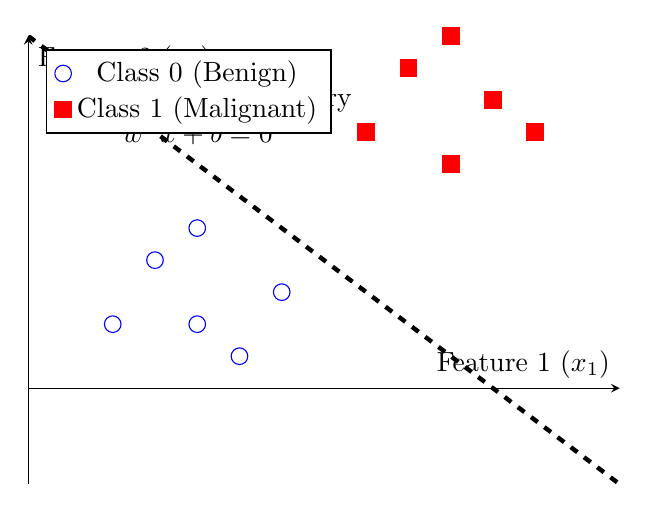
\begin{tikzpicture}
    \begin{axis}[
        xlabel={Feature 1 ($x_1$)},
        ylabel={Feature 2 ($x_2$)},
        axis lines=middle,
        width=0.75\textwidth,
        height=0.6\textwidth,
        xtick=\empty, ytick=\empty,
        legend pos=north west
    ]
    % Class 0 (Blue Circles)
    \addplot[only marks, mark=o, color=blue, mark size=3pt] coordinates {
        (1, 1) (1.5, 2) (2, 1) (2, 2.5) (3, 1.5) (2.5, 0.5)
    };
    \addlegendentry{Class 0 (Benign)}
    
    % Class 1 (Red Squares)
    \addplot[only marks, mark=square*, color=red, mark size=3pt] coordinates {
        (4, 4) (4.5, 5) (5, 3.5) (5.5, 4.5) (6, 4) (5, 5.5)
    };
    \addlegendentry{Class 1 (Malignant)}
    
    % Decision Boundary
    \addplot[domain=0:7, color=black, ultra thick, dashed] {-x + 5.5};
    \node[right] at (axis cs:1, 4.5) {Decision Boundary};
    \node[right] at (axis cs:1, 4) {$w^T x + b = 0$};
    \end{axis}
\end{tikzpicture}
\caption{Geometric View: The decision boundary separates the two classes.}
\label{fig:log_reg_geometry}
\end{figure}

The equation of this boundary is our familiar linear equation:
\begin{equation}
    z = w^T x + b = w_1 x_1 + w_2 x_2 + b
\end{equation}
\begin{itemize}
    \item If a point is on one side ($z > 0$), we predict Class 1.
    \item If a point is on the other side ($z < 0$), we predict Class 0.
    \item If $z = 0$, the point lies exactly on the boundary.
\end{itemize}

% ========================================
% SECTION: PERCEPTRON TRICK
% ========================================
\section{The Precursor: The Perceptron Trick}
Before Logistic Regression, there was the \textbf{Perceptron}. It uses a simple ``Push and Pull'' logic to find the decision boundary.

\subsection{The Algorithm}
\begin{enumerate}
    \item Start with a random line (random weights).
    \item Pick a random data point $(x_i, y_i)$.
    \item If it is \textbf{correctly classified}, do nothing.
    \item If it is \textbf{misclassified}:
    \begin{itemize}
        \item \textbf{Positive point in negative region}: Move the line \textit{towards} the point (Add $x_i$ to weights).
        \item \textbf{Negative point in positive region}: Move the line \textit{away} from the point (Subtract $x_i$ from weights).
    \end{itemize}
\end{enumerate}

\textbf{Unified Update Rule}:
\begin{equation}
    W_{\text{new}} = W_{\text{old}} + \eta (y_i - \hat{y}_i) x_i
\end{equation}

\subsection{Why did we move to Logistic Regression?}
The Perceptron has two major flaws:
\begin{enumerate}
    \item \textbf{No Conviction}: It stops as soon as points are separated, even if the line is barely touching the points. It doesn't find the \textit{best} line, just \textit{any} separating line.
    \item \textbf{Binary Output}: It gives a hard Yes/No, not a probability.
\end{enumerate}

\begin{lstlisting}[language=Python, caption=Perceptron Step Function]
import numpy as np

def perceptron_step(X, y, weights, lr=0.1):
    """Updates weights based on one random point."""
    idx = np.random.randint(0, X.shape[0])
    x_i, y_i = X[idx], y[idx]
    
    # Predict (Step Function)
    y_pred = 1 if np.dot(weights, x_i) >= 0 else 0
    
    # Update: W = W + lr * (y - y_pred) * x
    weights = weights + lr * (y_i - y_pred) * x_i
    return weights
\end{lstlisting}

% ========================================
% SECTION 4: THE SIGMOID FUNCTION
% ========================================
\section{The Sigmoid Function}
We need to convert the output $z$ (which ranges from $-\infty$ to $+\infty$) into a probability (range $[0, 1]$).

\begin{definition}
\textbf{Sigmoid Function} (also called Logistic Function):
\begin{equation}
    \sigma(z) = \frac{1}{1 + e^{-z}}
\end{equation}
\end{definition}

\begin{figure}[htbp]
\centering
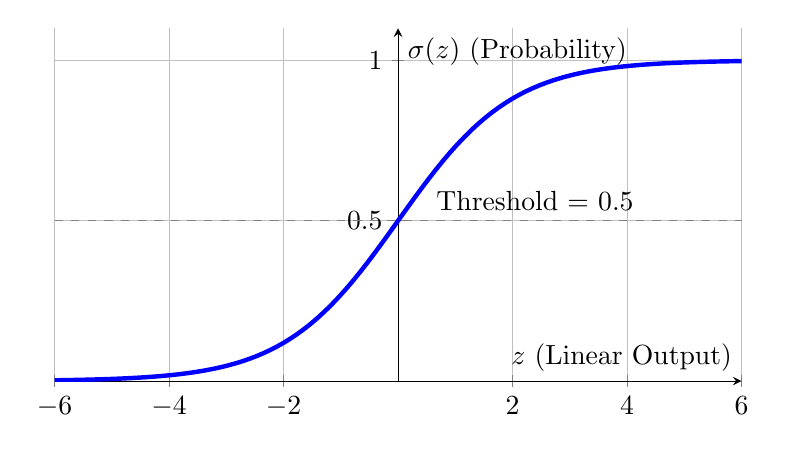
\begin{tikzpicture}
    \begin{axis}[
        xlabel={$z$ (Linear Output)},
        ylabel={$\sigma(z)$ (Probability)},
        xmin=-6, xmax=6,
        ymin=0, ymax=1.1,
        axis lines=middle,
        grid=major,
        width=0.85\textwidth,
        height=0.5\textwidth
    ]
    \addplot[domain=-6:6, color=blue, ultra thick, samples=100] {1/(1+exp(-x))};
    \draw[dashed, gray] (axis cs:-6, 0.5) -- (axis cs:6, 0.5);
    \node[above right] at (axis cs:0.5, 0.5) {Threshold = 0.5};
    \end{axis}
\end{tikzpicture}
\caption{The Sigmoid curve maps any real number to a valid probability between 0 and 1.}
\label{fig:sigmoid}
\end{figure}

\textbf{Key Properties}:
\begin{itemize}
    \item When $z=0$: $\sigma(z) = 0.5$ (Maximum uncertainty).
    \item When $z$ is large positive: $\sigma(z) \approx 1$ (Confident Class 1).
    \item When $z$ is large negative: $\sigma(z) \approx 0$ (Confident Class 0).
    \item The function is smooth and continuously differentiable.
\end{itemize}

% ========================================
% SECTION 5: POLYNOMIAL LOGISTIC REGRESSION
% ========================================
\section{Handling Non-Linear Data: Polynomial Features}
Standard Logistic Regression creates a \textbf{linear} decision boundary. But what if your data is shaped like a circle or a moon?

\textbf{The Trick}: We do NOT change the Logistic Regression algorithm. We change the \textbf{data} by adding polynomial features.

\textbf{Example}: If we have features $x_1$ and $x_2$, we add:
\begin{itemize}
    \item Degree 2: $x_1^2, x_2^2, x_1 \cdot x_2$
    \item Degree 3: $x_1^3, x_2^3, x_1^2 \cdot x_2, x_1 \cdot x_2^2$, etc.
\end{itemize}

The model still sees a linear equation: $z = w_1 x_1 + w_2 x_2 + w_3 x_1^2 + \ldots$

But in the \textit{original} 2D space, this creates a \textbf{curved decision boundary}.

\begin{lstlisting}[language=Python, caption=Polynomial Logistic Regression]
from sklearn.preprocessing import PolynomialFeatures
from sklearn.linear_model import LogisticRegression
from sklearn.pipeline import Pipeline
from sklearn.datasets import make_moons

# Create non-linear data (moon shapes)
X, y = make_moons(n_samples=200, noise=0.1)

# Pipeline: Polynomial Features -> Logistic Regression
model = Pipeline([
    ('poly', PolynomialFeatures(degree=3)),
    ('log_reg', LogisticRegression(max_iter=1000))
])

model.fit(X, y)
print(f"Accuracy: {model.score(X, y):.2f}")  # ~98%
\end{lstlisting}

\textbf{Warning}: High polynomial degrees (e.g., 10+) will \textbf{overfit}. Use cross-validation to find the optimal degree.

% ========================================
% SECTION 6: KEY TAKEAWAYS
% ========================================
\section{Key Takeaways}
\begin{enumerate}
    \item Logistic Regression is a \textbf{classification} algorithm, not regression.
    \item It finds a \textbf{linear decision boundary} to separate classes.
    \item The \textbf{Sigmoid function} converts the linear output to a probability.
    \item The model predicts the \textbf{probability} of belonging to a class, then thresholds at 0.5.
    \item For non-linear data, use \textbf{PolynomialFeatures} to create curved boundaries.
\end{enumerate}

% ========================================
% SECTION 7: HOTS QUESTIONS
% ========================================
\section{HOTS: Interview Questions}
\textbf{Q1: Why is it called ``Logistic Regression'' if it is used for classification?}
\begin{itemize}
    \item Historically, it was derived from regression techniques. The model ``regresses'' the log-odds (logit) of the probability, not the probability itself.
    \item $\text{logit}(p) = \log\left(\frac{p}{1-p}\right) = w^T x + b$
\end{itemize}

\textbf{Q2: Can Logistic Regression handle non-linear decision boundaries?}
\begin{itemize}
    \item By itself, no. It draws a straight line/hyperplane.
    \item However, you can engineer polynomial features (like $x_1^2, x_1 x_2$) to create curved boundaries.
\end{itemize}

\textbf{Q3: What happens if the data is perfectly linearly separable?}
\begin{itemize}
    \item The weights can grow infinitely large, trying to push the sigmoid output to exactly 0 or 1.
    \item Solution: Use \textbf{Regularization} (L2 penalty) to constrain the weights.
\end{itemize}

% ========================================
% SECTION 8: QUICK REFERENCE
% ========================================
\section{Quick Reference Card}

\begin{center}
\fbox{\parbox{0.9\textwidth}{
\textbf{LOGISTIC REGRESSION - CHEAT SHEET}
\vspace{0.3cm}

\textbf{Model}: $P(y=1|x) = \sigma(w^Tx + b) = \frac{1}{1+e^{-(w^Tx+b)}}$

\textbf{Decision Rule}: Predict Class 1 if $P > 0.5$, else Class 0

\textbf{Sigmoid Properties}:
\begin{itemize}
    \item $\sigma(0) = 0.5$ (Max uncertainty)
    \item $\sigma(\pm\infty) \rightarrow 0 \text{ or } 1$ (Confident)
    \item Derivative: $\sigma'(z) = \sigma(z)(1-\sigma(z))$
\end{itemize}

\textbf{Decision Boundary}: $w^Tx + b = 0$ (Linear hyperplane)

\textbf{Non-Linear Data}: Use \texttt{PolynomialFeatures} to curve the boundary

\textbf{Scikit-Learn}: \texttt{LogisticRegression(C=1.0, max\_iter=100)}

\textbf{Interview Gold}:
\begin{itemize}
    \item Name confusion: "Regression" is historical (regresses log-odds)
    \item Separable data $\rightarrow$ weights explode $\rightarrow$ use regularization
    \item Default boundary draws a straight line/hyperplane
\end{itemize}
}}

\chapter{The Loss Function: Binary Cross Entropy}
\label{chap:log_loss}

% ========================================
% SECTION 1: WHY NOT MSE?
% ========================================
\section{Why Not Mean Squared Error (MSE)?}
In Linear Regression, we used MSE as the loss function. Can we use it for Logistic Regression?
\begin{equation}
    J = \frac{1}{n} \sum (\sigma(z) - y)^2
\end{equation}
The answer is \textbf{No}. If you plot this loss function against the weights ($w$), it turns out to be \textbf{Non-Convex}.

\begin{itemize}
    \item It has many ``local minima'' (shallow valleys).
    \item Gradient Descent might get stuck in a local minimum instead of finding the global best solution.
\end{itemize}

\begin{figure}[htbp]
\centering
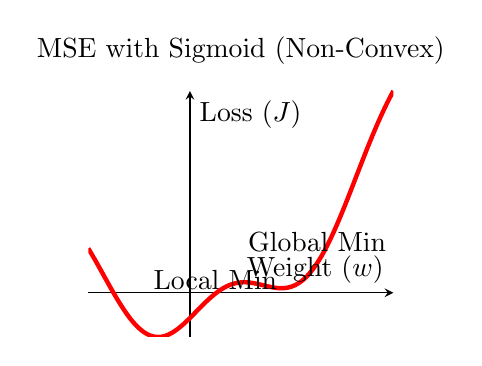
\begin{tikzpicture}
    \begin{axis}[
        xlabel={Weight ($w$)},
        ylabel={Loss ($J$)},
        ticks=none,
        axis lines=middle,
        width=0.45\textwidth,
        title={MSE with Sigmoid (Non-Convex)}
    ]
    \addplot[domain=-2:4, samples=100, smooth, ultra thick, color=red] {sin(deg(x*2)) + 0.5*x^2 - 1};
    \node at (axis cs:0.5, 0.5) {Local Min};
    \node at (axis cs:2.5, 2) {Global Min};
    \end{axis}
\end{tikzpicture}
\hfill
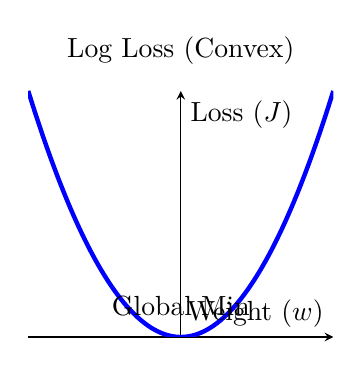
\begin{tikzpicture}
    \begin{axis}[
        xlabel={Weight ($w$)},
        ylabel={Loss ($J$)},
        ticks=none,
        axis lines=middle,
        width=0.45\textwidth,
        title={Log Loss (Convex)}
    ]
    \addplot[domain=-2:2, samples=100, smooth, ultra thick, color=blue] {x^2};
    \node at (axis cs:0, 0.5) {Global Min};
    \end{axis}
\end{tikzpicture}
\caption{Non-Convex (MSE) vs Convex (Log Loss). Gradient Descent is guaranteed to find the global minimum only for convex functions.}
\label{fig:convexity}
\end{figure}

% ========================================
% SECTION 2: MLE
% ========================================
\section{Maximum Likelihood Estimation (MLE)}
Instead of thinking about ``minimizing error'', we switch to a probabilistic view.

\begin{definition}
\textbf{Maximum Likelihood Estimation (MLE)}: A method to estimate model parameters by finding the values that \textbf{maximize the probability} of observing the given data.
\end{definition}

\textbf{Intuition}:
\begin{itemize}
    \item If a patient has cancer ($y=1$), we want our model to predict $\hat{y}$ close to 1.
    \item If a patient is healthy ($y=0$), we want $\hat{y}$ close to 0.
\end{itemize}

The \textbf{Likelihood} is the product of individual probabilities:
$$ L = \prod_{i=1}^{n} P(y_i | x_i; w) $$

\textbf{Problem}: Multiplying many small numbers ($0.9 \times 0.8 \times 0.7 \ldots$) leads to numerical underflow.

\textbf{Solution}: Take the \textbf{Logarithm}. Since $\log$ is monotonic, maximizing $\log(L)$ is equivalent to maximizing $L$.
$$ \log L = \sum_{i=1}^{n} \log P(y_i | x_i; w) $$

% ========================================
% SECTION 3: LOG LOSS
% ========================================
\section{Binary Cross Entropy (Log Loss)}
Since we want a \textbf{Loss Function} (to minimize), we take the \textbf{Negative} of the Log Likelihood.

\begin{definition}
\textbf{Binary Cross Entropy} (Log Loss):
\begin{equation}
    J(w) = - \frac{1}{n} \sum_{i=1}^{n} [ y_i \log(\hat{y}_i) + (1-y_i) \log(1 - \hat{y}_i) ]
\end{equation}
\end{definition}

\textbf{How it works}:
\begin{itemize}
    \item \textbf{Case 1: Actual $y = 1$}. The second term vanishes. Loss = $-\log(\hat{y})$.
        \begin{itemize}
            \item If $\hat{y} \approx 1$ (Correct): $-\log(1) = 0$ (No penalty).
            \item If $\hat{y} \approx 0$ (Wrong): $-\log(0) \rightarrow \infty$ (Huge penalty).
        \end{itemize}
    \item \textbf{Case 2: Actual $y = 0$}. The first term vanishes. Loss = $-\log(1-\hat{y})$.
        \begin{itemize}
            \item If $\hat{y} \approx 0$ (Correct): $-\log(1) = 0$.
            \item If $\hat{y} \approx 1$ (Wrong): $-\log(0) \rightarrow \infty$.
        \end{itemize}
\end{itemize}

% ========================================
% SECTION 4: SIGMOID DERIVATIVE
% ========================================
\section{Derivative of the Sigmoid Function}
To apply Gradient Descent, we need the derivative of the Sigmoid.

\begin{equation}
    \sigma(z) = \frac{1}{1 + e^{-z}}
\end{equation}

Using the chain rule and simplifying (derivation in source notes):
\begin{equation}
    \boxed{\frac{d\sigma}{dz} = \sigma(z) \cdot (1 - \sigma(z))}
\end{equation}

This elegant result makes gradient calculations very clean.

% ========================================
% SECTION 5: GRADIENT DESCENT UPDATE
% ========================================
\section{Gradient Descent for Logistic Regression}
Unlike Linear Regression, Logistic Regression has \textbf{no closed-form solution}. We must use iterative optimization.

The gradient of the Log Loss with respect to weights $w$ simplifies to:
\begin{equation}
    \frac{\partial J}{\partial w_j} = \frac{1}{n} \sum_{i=1}^{n} (\hat{y}_i - y_i) x_{ij}
\end{equation}

This is remarkably similar to Linear Regression. The update rule is:
\begin{equation}
    w_j := w_j - \eta \cdot \frac{1}{n} \sum_{i=1}^{n} (\hat{y}_i - y_i) x_{ij}
\end{equation}

% ========================================
% SECTION 6: HOTS
% ========================================
\section{HOTS: Interview Questions}
\textbf{Q1: Why is Log Loss convex but MSE with Sigmoid is not?}
\begin{itemize}
    \item The Sigmoid function is non-linear. When you square the difference $(\sigma(z) - y)^2$, the resulting surface has multiple bumps.
    \item Log Loss is mathematically designed (via MLE) to be convex for the Sigmoid output.
\end{itemize}

\textbf{Q2: What is the relationship between Cross Entropy and KL Divergence?}
\begin{itemize}
    \item Cross Entropy measures the dissimilarity between two probability distributions.
    \item KL Divergence = Cross Entropy - Entropy of the true distribution.
    \item Minimizing Cross Entropy is equivalent to minimizing KL Divergence when the true distribution is fixed.
\end{itemize}

\chapter{Classification Metrics}
\label{chap:classification_metrics}

% ========================================
% SECTION 1: INTRODUCTION
% ========================================
\section{Introduction: Why Accuracy is Not Enough}
Accuracy ($\frac{\text{Correct Predictions}}{\text{Total Predictions}}$) is a dangerous metric.

\textbf{Example}: Imagine a dataset with 99 healthy patients and 1 cancer patient.
\begin{itemize}
    \item A lazy model predicts ``Healthy'' for everyone.
    \item Accuracy = $\frac{99}{100} = 99\%$.
    \item But it killed the one patient it needed to save. It is a \textbf{useless model}.
\end{itemize}

We need metrics that account for the \textbf{type} of errors, not just the count.

% ========================================
% SECTION 2: CONFUSION MATRIX
% ========================================
\section{The Confusion Matrix}
We break down predictions into 4 buckets:

\begin{table}[htbp]
    \centering
    \begin{tabular}{|l|c|c|}
    \hline
    & \textbf{Predicted Positive (1)} & \textbf{Predicted Negative (0)} \\ \hline
    \textbf{Actual Positive (1)} & True Positive (TP) & False Negative (FN) \\ \hline
    \textbf{Actual Negative (0)} & False Positive (FP) & True Negative (TN) \\ \hline
    \end{tabular}
    \caption{The Confusion Matrix for Binary Classification}
    \label{tab:confusion_matrix}
\end{table}

\textbf{How to Remember TP/TN/FP/FN}:
\begin{itemize}
    \item \textbf{First Letter (T/F)}: Was the prediction correct? (True = Yes, False = No)
    \item \textbf{Second Letter (P/N)}: What was the predicted class? (Positive or Negative)
\end{itemize}

\textbf{Error Types}:
\begin{itemize}
    \item \textbf{Type I Error (FP)}: ``False Alarm''. Example: A man told he is pregnant.
    \item \textbf{Type II Error (FN)}: ``Missed Detection''. Example: A pregnant woman told she is not pregnant.
\end{itemize}

\begin{figure}[htbp]
\centering
\includegraphics[width=0.7\textwidth]{../02-supervised/assets/confusion_matrix_visual.png}
\caption{Visual representation of the Confusion Matrix components.}
\label{fig:confusion_visual}
\end{figure}

% ========================================
% SECTION 3: PRECISION
% ========================================
\section{Precision: ``Out of My Positive Claims, How Many Were Right?''}
\begin{definition}
\textbf{Precision}: Out of all instances \textit{predicted} as Positive, how many were \textit{actually} Positive?
\begin{equation}
    \text{Precision} = \frac{TP}{TP + FP}
\end{equation}
\end{definition}

\textbf{Scenario: Spam Filter}.
\begin{itemize}
    \item \textbf{FP is costly}: A real email from your boss is marked as Spam. (Disaster).
    \item \textbf{Goal}: We want to be very sure before flagging something as Spam. We need \textbf{High Precision}.
\end{itemize}

% ========================================
% SECTION 4: RECALL
% ========================================
\section{Recall: ``Out of All Actual Positives, How Many Did I Find?''}
\begin{definition}
\textbf{Recall} (Sensitivity, True Positive Rate): Out of all \textit{actual} Positive instances, how many did the model capture?
\begin{equation}
    \text{Recall} = \frac{TP}{TP + FN}
\end{equation}
\end{definition}

\textbf{Scenario: Cancer Detection}.
\begin{itemize}
    \item \textbf{FN is fatal}: A sick patient is told they are healthy.
    \item \textbf{FP is okay}: A healthy person undergoes extra tests. (Annoying but safe).
    \item \textbf{Goal}: We cannot afford to miss any cancer case. We need \textbf{High Recall}.
\end{itemize}

\begin{figure}[htbp]
\centering
\includegraphics[width=0.45\textwidth]{../02-supervised/assets/precision_spam_visual.png}
\hfill
\includegraphics[width=0.45\textwidth]{../02-supervised/assets/recall_cancer_visual.png}
\caption{Left: Precision matters in Spam detection (avoid FP). Right: Recall matters in Cancer detection (avoid FN).}
\label{fig:precision_recall_visual}
\end{figure}

% ========================================
% SECTION 5: F1-SCORE
% ========================================
\section{F1-Score: The Balanced Metric}
Often, we need a balance. Simple average is biased. We use the \textbf{Harmonic Mean}.

\begin{definition}
\textbf{F1-Score}: The harmonic mean of Precision and Recall.
\begin{equation}
    \text{F1} = 2 \times \frac{\text{Precision} \times \text{Recall}}{\text{Precision} + \text{Recall}} = \frac{2 \cdot TP}{2 \cdot TP + FP + FN}
\end{equation}
\end{definition}

\textbf{Why Harmonic Mean?}: It penalizes extreme values. If Precision=1.0 and Recall=0.0:
\begin{itemize}
    \item Arithmetic Mean: $(1.0 + 0.0)/2 = 0.5$ (Misleading).
    \item Harmonic Mean: $2 \times \frac{1.0 \times 0.0}{1.0 + 0.0} = 0$ (Correct - model is useless).
\end{itemize}

% ========================================
% SECTION 6: ROC-AUC
% ========================================
\section{ROC-AUC: Threshold-Independent Metric}
All the above metrics depend on choosing a threshold (default 0.5). The \textbf{ROC Curve} evaluates performance across \textit{all possible thresholds}.

\begin{definition}
\textbf{ROC Curve} (Receiver Operating Characteristic): A plot of True Positive Rate (Recall) vs False Positive Rate at various threshold settings.
\begin{equation}
    \text{FPR} = \frac{FP}{FP + TN} = \frac{\text{False Alarms}}{\text{Total Actual Negatives}}
\end{equation}
\end{definition}

\begin{definition}
\textbf{AUC} (Area Under the Curve): The area under the ROC curve. Ranges from 0 to 1.
\begin{itemize}
    \item AUC = 1.0: Perfect classifier.
    \item AUC = 0.5: Random guessing (diagonal line).
    \item AUC $<$ 0.5: Worse than random (invert predictions).
\end{itemize}
\end{definition}

% (Moved to Chapter 9)

% ========================================
% SECTION 8: IMPLEMENTATION
% ========================================
\section{Implementation in Python}
\begin{lstlisting}[language=Python, caption=Classification Metrics with Scikit-Learn]
from sklearn.metrics import (
    classification_report, confusion_matrix,
    precision_score, recall_score, f1_score, roc_auc_score
)
from sklearn.datasets import load_iris
from sklearn.model_selection import train_test_split
from sklearn.linear_model import LogisticRegression

# Load and split data
X, y = load_iris(return_X_y=True)
X_train, X_test, y_train, y_test = train_test_split(X, y, test_size=0.3)

# Train model
model = LogisticRegression(max_iter=200)
model.fit(X_train, y_train)
y_pred = model.predict(X_test)

# 1. Confusion Matrix
print("Confusion Matrix:")
print(confusion_matrix(y_test, y_pred))

# 2. Classification Report (All metrics at once)
print("\nClassification Report:")
print(classification_report(y_test, y_pred, 
      target_names=['Setosa', 'Versicolor', 'Virginica']))

# 3. Specific Averaging
print(f"Macro F1: {f1_score(y_test, y_pred, average='macro'):.3f}")
print(f"Weighted F1: {f1_score(y_test, y_pred, average='weighted'):.3f}")
\end{lstlisting}

\textbf{Sample Output}:
\begin{verbatim}
              precision    recall  f1-score   support
     Setosa       1.00      1.00      1.00        15
 Versicolor       0.94      0.90      0.92        18
  Virginica       0.88      0.93      0.90        12
   accuracy                           0.93        45
  macro avg       0.94      0.94      0.94        45
weighted avg      0.94      0.93      0.93        45
\end{verbatim}

% ========================================
% SECTION 9: SUMMARY TABLE
% ========================================
\section{Summary: When to Use Which Metric}
\begin{center}
\begin{tabular}{|l|l|l|}
\hline
\textbf{Metric} & \textbf{Use When...} & \textbf{Example} \\ \hline
Accuracy & Classes are balanced & General purpose \\ \hline
Precision & FP is costly & Spam filter, Legal \\ \hline
Recall & FN is costly & Cancer, Fraud detection \\ \hline
F1-Score & Need balance & Most imbalanced datasets \\ \hline
ROC-AUC & Comparing models & Model selection \\ \hline
Macro F1 & All classes equal & Rare disease classes \\ \hline
Weighted F1 & Account for imbalance & Production systems \\ \hline
\end{tabular}
\end{center}

% ========================================
% SECTION 10: HOTS QUESTIONS
% ========================================
\section{HOTS: Interview Questions}
\textbf{Q1: What is the difference between Macro and Weighted F1?}
\begin{itemize}
    \item Macro F1 gives equal weight to each class, regardless of size.
    \item Weighted F1 weights each class by its number of samples.
    \item Use Macro when minority classes are important; use Weighted for overall performance.
\end{itemize}

\textbf{Q2: How do you calculate Precision for a specific class in multiclass?}
\begin{itemize}
    \item Treat it as ``Class $c$ vs Rest''.
    \item TP = correctly predicted as $c$.
    \item FP = incorrectly predicted as $c$ (was actually another class).
    \item Precision$_c$ = TP / (TP + FP).
\end{itemize}

\textbf{Q3: Why is ROC-AUC not suitable for highly imbalanced data?}
\begin{itemize}
    \item ROC uses FPR which can be low even when FP is high (if TN is very large).
    \item For imbalanced data, use PR-AUC (Precision-Recall AUC) instead.
\end{itemize}

% ========================================
% SECTION 11: QUICK REFERENCE
% ========================================
\section{Quick Reference Card}

\begin{center}
\fbox{\parbox{0.9\textwidth}{
\textbf{CLASSIFICATION METRICS - CHEAT SHEET}
\vspace{0.3cm}

\textbf{Core Formulas}:
\begin{itemize}
    \item Precision = $\frac{TP}{TP+FP}$ (How many positive claims were right?)
    \item Recall = $\frac{TP}{TP+FN}$ (How many positives did we find?)
    \item F1 = $\frac{2 \cdot P \cdot R}{P + R}$ (Harmonic mean)
    \item Accuracy = $\frac{TP+TN}{All}$ (Misleading for imbalanced data!)
\end{itemize}

\textbf{When to Use What}:
\begin{center}
\begin{tabular}{|l|l|}
\hline
\textbf{Scenario} & \textbf{Metric} \\ \hline
Spam filter (avoid false alarms) & Precision \\ \hline
Cancer detection (don't miss cases) & Recall \\ \hline
Balanced tradeoff & F1-Score \\ \hline
Model comparison & ROC-AUC \\ \hline
Imbalanced data & PR-AUC \\ \hline
\end{tabular}
\end{center}

\textbf{Interview Gold}:
\begin{itemize}
    \item Accuracy trap: 99\% accuracy can be useless
    \item F1 uses harmonic mean: penalizes extremes
    \item ROC plots TPR vs FPR across all thresholds
\end{itemize}
}}

\part{Decision Trees}
\chapter{Decision Trees: Intuition and Geometry}
\label{chap:decision_tree_intuition}

\section{Introduction}
In previous chapters, we studied Linear Models (Linear Regression, Logistic Regression, SVM) which try to find a mathematical equation (a line or hyperplane) to separate data.
\textbf{Decision Trees} take a completely different approach. Instead of finding a complex formula, they ask a series of simple questions.

\begin{definition}
\textbf{Decision Tree}: A hierarchical Supervised Learning model that splits data into subsets based on the value of input features. It mimics human decision-making by asking a sequence of "if-else" questions to arrive at a prediction.
\end{definition}

\section{The Intuition: The "20 Questions" Game}
Imagine you are playing a game with a friend. You have to guess the animal they are thinking of, but you are only allowed to ask \textbf{Yes/No} questions.

\begin{itemize}
    \item \textbf{Question 1}: Is it bigger than a cat?
    \begin{itemize}
        \item \textit{Answer}: No. (You immediately rule out Elephants, Tigers, etc.)
    \end{itemize}
    \item \textbf{Question 2}: Does it fly?
    \begin{itemize}
        \item \textit{Answer}: Yes. (You assume it's a bird or insect).
    \end{itemize}
    \item \textbf{Question 3}: Is it green?
    \begin{itemize}
        \item \textit{Answer}: Yes.
    \end{itemize}
    \item \textbf{Conclusion}: It is a \textbf{Parrot}.
\end{itemize}

This is exactly how a Decision Tree works.
\begin{enumerate}
    \item The entire dataset starts at the \textbf{Root Node}.
    \item The algorithm picks the "Question" (Feature) that divides the data most effectively.
    \item It repeats this process until it reaches a conclusion (\textbf{Leaf Node}).
\end{enumerate}

\section{Geometric Intuition: Space Cutting}
To understand Decision Trees mathematically, we must view them as \textbf{Space Cutters}.
\begin{itemize}
    \item Review: \textbf{Linear Regression} draws a single diagonal line: $y = mx + c$.
    \item **Decision Trees** cannot draw diagonals. They draw \textbf{Orthogonal Cuts} (lines parallel to the X or Y axes).
\end{itemize}

\begin{itemize}
    \item If the rule is $X < 5$, it draws a vertical line at $X=5$.
    \item If the next rule is $Y < 3$, it draws a horizontal line at $Y=3$ \textit{within that region}.
\end{itemize}

By making these repeated vertical and horizontal cuts, the Tree divides the entire N-dimensional feature space into rectangular regions called \textbf{Hyper-cuboids}.

\begin{figure}[htbp]
\centering
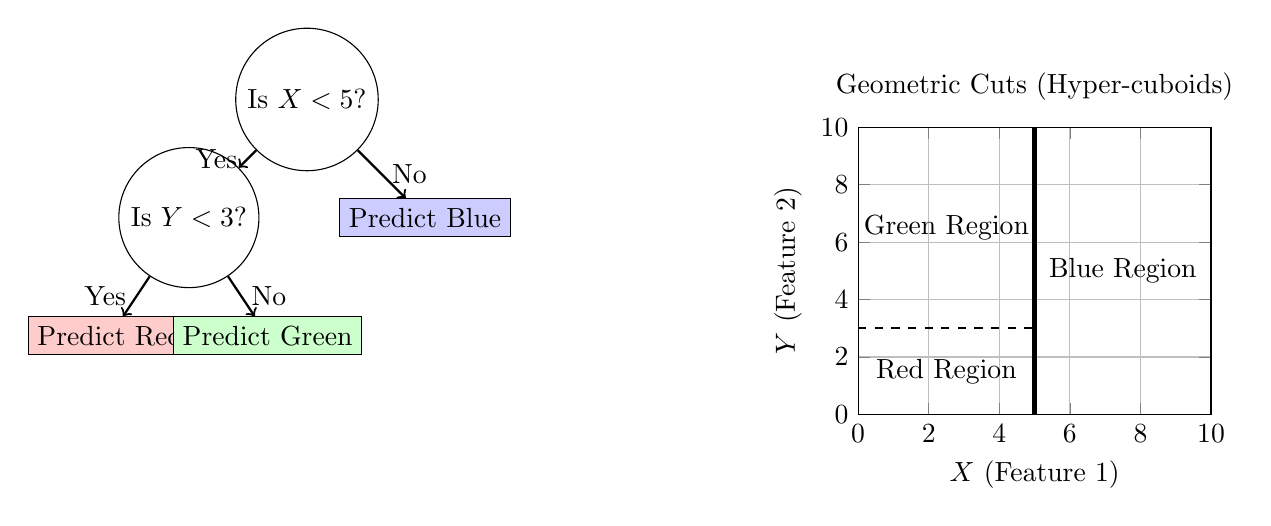
\begin{tikzpicture}
    % Tree Structure (Left)
    \node (root) at (-4, 2) [circle, draw, align=center] {Is $X < 5$?};
    \node (node1) at (-5.5, 0.5) [circle, draw, align=center] {Is $Y < 3$?};
    \node (leaf1) at (-2.5, 0.5) [rectangle, draw, fill=blue!20, minimum width=1.5cm] {Predict Blue};
    \node (leaf2) at (-6.5, -1) [rectangle, draw, fill=red!20, minimum width=1.5cm] {Predict Red};
    \node (leaf3) at (-4.5, -1) [rectangle, draw, fill=green!20, minimum width=1.5cm] {Predict Green};
    
    \draw[->, thick] (root) -- node[left] {Yes} (node1);
    \draw[->, thick] (root) -- node[right] {No} (leaf1);
    \draw[->, thick] (node1) -- node[left] {Yes} (leaf2);
    \draw[->, thick] (node1) -- node[right] {No} (leaf3);
    
    % Geometric Space (Right)
    \begin{axis}[
        at={(3cm,-2cm)},
        width=0.5\textwidth,
        xmin=0, xmax=10, ymin=0, ymax=10,
        xlabel=$X$ (Feature 1), ylabel=$Y$ (Feature 2),
        title={Geometric Cuts (Hyper-cuboids)},
        grid=major
    ]
        % Vertical Cut X=5
        \draw[ultra thick] (axis cs:5, 0) -- (axis cs:5, 10);
        \node at (axis cs:7.5, 5) {Blue Region};
        
        % Horizontal Cut Y=3 (Only where X < 5)
        \draw[thick, dashed] (axis cs:0, 3) -- (axis cs:5, 3);
        
        \node at (axis cs:2.5, 1.5) {Red Region};
        \node at (axis cs:2.5, 6.5) {Green Region};
    \end{axis}
\end{tikzpicture}
\caption{Left: The Logic flow (Tree). Right: The Geometry showing how logic converts to rectangular regions.}
\label{fig:tree_geometry}
\end{figure}

\section{Terminology}
Let us formalize the parts of a tree:
\begin{enumerate}
    \item \textbf{Root Node}: The top-most node. It contains the entire dataset ($100\%$ of samples) before any splitting happens.
    \item \textbf{Decision Node} (Internal Node): A node that splits the data further based on a condition.
    \item \textbf{Leaf Node} (Terminal Node): A node that does not split. It contains the final prediction (e.g., "This is a Cat").
    \item \textbf{Splitting}: The process of dividing a node into two or more sub-nodes.
    \item \textbf{Pruning}: The process of removing branches to reduce the size of the decision tree and prevent Overfitting.
\end{enumerate}

\section{Implementation in Python}
\begin{lstlisting}[language=Python, caption=Basic Decision Tree Classifier]
from sklearn.datasets import load_iris
from sklearn.tree import DecisionTreeClassifier, plot_tree
from sklearn.model_selection import train_test_split
import matplotlib.pyplot as plt

# Load Data
X, y = load_iris(return_X_y=True)
X_train, X_test, y_train, y_test = train_test_split(X, y, test_size=0.2)

# Train Decision Tree
tree = DecisionTreeClassifier(max_depth=3, random_state=42)
tree.fit(X_train, y_train)

# Visualize the Tree
plt.figure(figsize=(12, 8))
plot_tree(tree, filled=True, feature_names=load_iris().feature_names)
plt.title("Decision Tree Visualization")
plt.show()

print(f"Accuracy: {tree.score(X_test, y_test):.2f}")
\end{lstlisting}

\section{HOTS: Interview Questions}
\textbf{Q1: Can Decision Trees draw diagonal decision boundaries?}
\begin{itemize}
    \item No. By design, they only make cuts parallel to the axes (orthogonal cuts). To approximate a diagonal, they would need many staircase-like splits.
\end{itemize}

\textbf{Q2: Why are Decision Trees called ``Greedy'' algorithms?}
\begin{itemize}
    \item At each node, the tree picks the \textit{locally} best split (maximum Information Gain). It does not look ahead to see if a different split would be globally better. This makes it fast but potentially suboptimal.
\end{itemize}

% ========================================
% SECTION: QUICK REFERENCE
% ========================================
\section{Quick Reference Card}

\begin{center}
\fbox{\parbox{0.9\textwidth}{
\textbf{DECISION TREES - CHEAT SHEET}
\vspace{0.3cm}

\textbf{Core Idea}: Game of ``20 Questions'' - split data with yes/no questions

\textbf{Geometry}: Orthogonal cuts create axis-parallel hyper-cuboid regions

\textbf{Key Terminology}:
\begin{itemize}
    \item \textbf{Root}: First decision node
    \item \textbf{Leaf}: Terminal node with prediction
    \item \textbf{Depth}: Longest path from root to leaf
\end{itemize}

\textbf{Splitting Criteria}:
\begin{itemize}
    \item Classification: Entropy, Gini Impurity
    \item Regression: Variance Reduction (MSE)
\end{itemize}

\textbf{Sklearn}: \texttt{DecisionTreeClassifier(max\_depth=5)}

\textbf{Interview Gold}:
\begin{itemize}
    \item Greedy: picks locally best split (not globally optimal)
    \item Cannot draw diagonal boundaries (only orthogonal)
    \item No scaling needed! (based on thresholds, not distances)
\end{itemize}
}}

\chapter{Splitting Metrics: Entropy and Gini}
\label{chap:splitting_metrics}

\section{The Core Problem: How to Split?}
A Decision Tree makes thousands of cuts. But how does it decide \textit{where} to cut?
Should it split on "Age" or "Income"? Should the threshold be 25 years or 30 years?
\\ To answer this, we need a mathematical way to measure the quality of a split. The goal is to maximize \textbf{Purity}.

\begin{definition}
\textbf{Purity}: A node is "Pure" if it contains samples from only one class (e.g., 100\% Cats). It is "Impure" if it is a mix (e.g., 50\% Cats, 50\% Dogs).
\end{definition}

\section{Entropy (Measure of Surprise)}
Entropy is a concept borrowed from Physics (Thermodynamics) and Information Theory.
\begin{definition}
\textbf{Entropy ($H$)}: A measure of randomness or disorder in a set of data. In Machine Learning, it measures impurity.
\end{definition}

\begin{itemize}
    \item **High Entropy**: High disorder (e.g., A coin flip is 50/50. You are maximally "Surprised" by the outcome).
    \item **Low Entropy**: Low disorder (e.g., An unfair coin that is Heads 99\% of the time. You are not surprised).
\end{itemize}

\subsection{Mathematical Formula}
For a binary classification problem ($p_+$ is probability of Positive, $p_-$ is probability of Negative):
\begin{equation}
    H(S) = - p_+ \log_2(p_+) - p_- \log_2(p_-)
\end{equation}

\subsection{Example Calculation}
Imagine a node with 5 animals: \textbf{2 Cats, 3 Dogs}.
\begin{enumerate}
    \item Probability of Cat ($p_+$) = $2/5 = 0.4$
    \item Probability of Dog ($p_-$) = $3/5 = 0.6$
    \item Calculate Entropy:
\end{enumerate}
$$ H = - [ (0.4 \log_2 0.4) + (0.6 \log_2 0.6) ] $$
$$ \log_2(0.4) \approx -1.32, \quad \log_2(0.6) \approx -0.73 $$
$$ H = - [ (0.4 \times -1.32) + (0.6 \times -0.73) ] $$
$$ H = - [ -0.528 - 0.438 ] = - [-0.966] \approx \mathbf{0.97} $$
\textbf{Conclusion}: $0.97$ is very close to 1. This node is highly impure.

\section{Information Gain}
Identifying impurity is not enough. We want to \textit{reduce} it.
\begin{definition}
\textbf{Information Gain}: The reduction in Entropy after splitting a node on a particular attribute.
\end{definition}
\begin{equation}
    \text{Gain} = H(\text{Parent}) - \sum \frac{N_{\text{child}}}{N_{\text{parent}}} H(\text{Child})
\end{equation}
The algorithm calculates the Information Gain for every possible split and chooses the one with the \textbf{Highest Gain}.

\section{Gini Impurity}
While Entropy is conceptually beautiful, calculating Logarithms ($\log_2$) is computationally expensive for computers.
Most modern libraries (like Scikit-Learn's CART) use \textbf{Gini Impurity} by default.

\begin{definition}
\textbf{Gini Impurity}: A measure of how often a randomly chosen element from the set would be incorrectly labeled.
\end{definition}
\begin{equation}
    \text{Gini} = 1 - \sum_{i=1}^{K} p_i^2
\end{equation}

\textbf{Gini vs Entropy}:
\begin{itemize}
    \item \textbf{Gini}: Max value is 0.5. Computationally faster (squaring is easy).
    \item \textbf{Entropy}: Max value is 1.0. Slower.
    \item \textit{Practical Note}: In 99\% of cases, they yield the same tree. Stick to Gini for speed.
\end{itemize}

\begin{figure}[htbp]
\centering
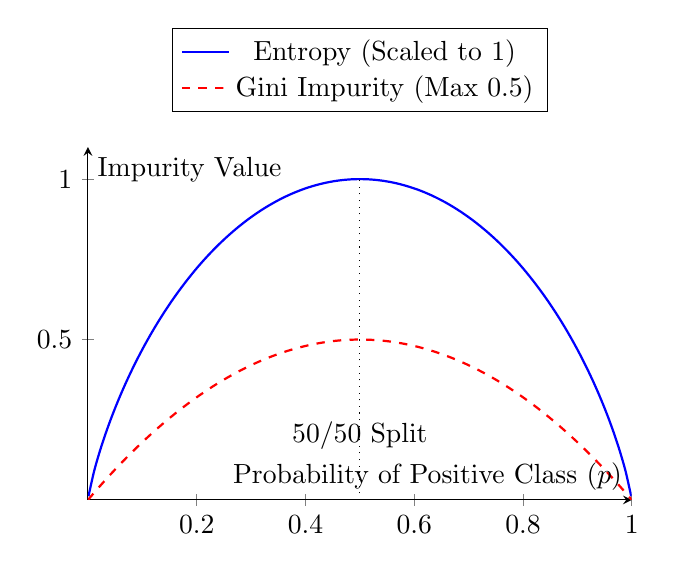
\begin{tikzpicture}
    \begin{axis}[
        xlabel={Probability of Positive Class ($p$)},
        ylabel={Impurity Value},
        xmin=0, xmax=1,
        ymin=0, ymax=1.1,
        axis lines=middle,
        width=0.7\textwidth,
        height=0.5\textwidth,
        legend style={at={(0.5,1.1)},anchor=south}
    ]
    % Entropy Curve
    \addplot[domain=0.001:0.999, samples=100, smooth, thick, blue] {-x*ln(x)/ln(2) - (1-x)*ln(1-x)/ln(2)};
    \addlegendentry{Entropy (Scaled to 1)}
    
    % Gini Curve (Scaled to match height roughly for comparison? No, plot actual Gini)
    \addplot[domain=0:1, samples=100, smooth, thick, red, dashed] {1 - (x^2 + (1-x)^2)};
    \addlegendentry{Gini Impurity (Max 0.5)}
    
    \draw[dotted] (axis cs:0.5, 0) -- (axis cs:0.5, 1);
    \node at (axis cs:0.5, 0.2) {50/50 Split};
    \end{axis}
\end{tikzpicture}
\caption{Comparison of Entropy and Gini. Both are maximized at $p=0.5$ (Maximum uncertainty).}
\label{fig:entropy_gini}
\end{figure}

\section{HOTS: Interview Questions}
\textbf{Q1: What is the difference between Entropy and Gini Impurity?}
\begin{itemize}
    \item Entropy uses logarithms; Gini uses simple squaring.
    \item Entropy ranges from 0 to 1; Gini ranges from 0 to 0.5 (for binary).
    \item In practice, they usually produce identical trees.
\end{itemize}

\textbf{Q2: Why is Information Gain sometimes biased towards features with many values?}
\begin{itemize}
    \item If a feature has many unique values (e.g., ``Customer ID'' with 1000 values), splitting on it creates very ``pure'' leaves (each leaf has one customer). 
    \item This leads to high Information Gain but severe overfitting.
    \item Solution: Use Gain Ratio (C4.5) or Gini (CART).
\end{itemize}

% ========================================
% SECTION: QUICK REFERENCE
% ========================================
\section{Quick Reference Card}

\begin{center}
\fbox{\parbox{0.9\textwidth}{
\textbf{SPLITTING METRICS - CHEAT SHEET}
\vspace{0.3cm}

\textbf{Entropy} (Information Theory):
$$H = -\sum_{i=1}^{K} p_i \log_2(p_i)$$
Range: 0 (pure) to $\log_2(K)$ (max uncertainty)

\textbf{Gini Impurity} (Probability-based):
$$Gini = 1 - \sum_{i=1}^{K} p_i^2$$
Range: 0 (pure) to $1 - 1/K$ (For binary: max 0.5)

\textbf{Information Gain}:
$$IG = H_{parent} - \sum \frac{n_{child}}{n_{parent}} H_{child}$$

\textbf{Comparison}:
\begin{center}
\begin{tabular}{|l|l|}
\hline
\textbf{Entropy} & Uses log, slightly slower \\ \hline
\textbf{Gini} & Faster, default in sklearn \\ \hline
\textbf{Trees?} & Usually identical \\ \hline
\end{tabular}
\end{center}

\textbf{Interview Gold}:
\begin{itemize}
    \item Pure node = Entropy/Gini = 0
    \item 50/50 split = maximum impurity
    \item IG bias: use Gain Ratio for many-valued features
\end{itemize}
}}

\chapter{Tree Algorithms: ID3 vs CART}
\label{chap:tree_algorithms}

\section{Evolution of Tree Algorithms}
Decision Trees are not a single algorithm but a family of algorithms. The most famous ones are ID3, C4.5, and CART.

\section{ID3 (Iterative Dichotomiser 3)}
Developed by Ross Quinlan in 1986. It was the first widely used algorithm.
\begin{itemize}
    \item **Metric**: Uses \textbf{Entropy} and Information Gain.
    \item **Structure**: It creates \textbf{Multi-way Splits}. If a feature "Color" has 3 values (Red, Green, Blue), ID3 creates 3 child nodes immediately.
    \item **Start Limitation**: It could not handle numerical features (e.g., Salary) directly; they had to be converted into categories (Low, Med, High).
\end{itemize}

\section{CART (Classification And Regression Trees)}
This is the modern standard and the algorithm used by Python's Scikit-Learn.

\begin{definition}
\textbf{CART}: A flexible tree algorithm that constructs strictly \textbf{Binary Trees} (only 2 children per node). It supports both Classification (using Gini) and Regression (using MSE).
\end{definition}

\subsection{Key Differences}
\begin{table}[h!]
\centering
\begin{tabular}{|l|l|l|}
\hline
\textbf{Feature} & \textbf{ID3 / C4.5} & \textbf{CART (Scikit-Learn)} \\ \hline
\textbf{Splitting Criteria} & Entropy (Info Gain) & Gini Impurity (Default) \\ \hline
\textbf{Structure} & Multi-way Tree (Variable branches) & Binary Tree (Always Yes/No) \\ \hline
\textbf{Numerical Data} & Poor support (ID3) & Full support (Sort \& Threshold) \\ \hline
\textbf{Task} & Classification Only & Classification \& Regression \\ \hline
\end{tabular}
\caption{Comparison of classic ID3 vs modern CART.}
\label{tab:id3_vs_cart}
\end{table}

\section{Decision Trees for Regression}
It may seem counter-intuitive that a tree (which outputs "Classes") can predict a number.
\begin{itemize}
    \item **Splitting**: Instead of minimizing Impurity (Gini), it minimizes \textbf{Variance} (Mean Squared Error).
    \item **Prediction**: The prediction for a Leaf Node is not a "Vote", but the \textbf{Mean Average} of all training samples in that leaf.
\end{itemize}

\begin{definition}
\textbf{Step Function}: The output of a Regression Tree is not a smooth curve. It is a series of flat steps (Piecewise Constant). $y = \text{mean}(Leaf_1)$ if $x \in R_1$, etc.
\end{definition}

\section{Implementation in Python}
\begin{lstlisting}[language=Python, caption=Regression Tree Example]
from sklearn.tree import DecisionTreeRegressor
import numpy as np

# Create simple data
X = np.arange(1, 11).reshape(-1, 1)
y = np.array([1.5, 1.7, 1.9, 5.0, 5.2, 5.5, 8.0, 8.2, 8.5, 9.0])

# Fit Regression Tree
tree = DecisionTreeRegressor(max_depth=2)
tree.fit(X, y)

# Predictions are step-wise constant
print(tree.predict([[2.5], [6], [9.5]]))  # Output: flat values per region
\end{lstlisting}

\section{HOTS: Interview Questions}
\textbf{Q1: What is the key difference between ID3 and CART?}
\begin{itemize}
    \item ID3 creates multi-way splits and only handles categorical data.
    \item CART always creates binary splits and handles both numerical and categorical data.
\end{itemize}

\textbf{Q2: How does a Regression Tree make predictions?}
\begin{itemize}
    \item It predicts the \textbf{mean} of the target values for all training samples that fall into that leaf.
    \item This results in a step-function (piecewise constant) prediction surface.
\end{itemize}

\chapter{Overfitting and Pruning}
\label{chap:pruning}

\section{The Tree's Achilles Heel: Overfitting}
Decision Trees are aggressive learners. If left unchecked, they will split the data until every single leaf node is "Pure".
\begin{itemize}
    \item Imagine a leaf node containing just \textbf{1 person} who is an outlier (e.g., a smoker who lived to 100).
    \item The tree learns a rule: "If you smoke and live in this specific zip code $\rightarrow$ You live to 100".
    \item This is \textbf{Overfitting}. The tree memorizes the training noise.
\end{itemize}

\begin{definition}
\textbf{Pruning}: The technique of reducing the size of a decision tree by removing sections that provide little power to classify instances. It allows the tree to generalize better.
\end{definition}

\section{Pre-Pruning (Early Stopping)}
We stop the tree \textit{while} it is growing. This is done using Hyperparameters.

\begin{itemize}
    \item \texttt{max\_depth}: Constraint the tree height (e.g., max 5 levels).
    \item \texttt{min\_samples\_split}: "Don't split this node unless it has at least 50 people".
    \item \texttt{min\_samples\_leaf}: "Don't create a leaf unless it has at least 10 people". (Crucial for smoothing).
\end{itemize}

\section{Post-Pruning (Cost Complexity Pruning)}
Pre-pruning is basically guessing parameters. A more mathematical approach is to let the tree grow fully (to 100\% purity), and then cut off the "weakest" branches.
Scikit-Learn uses **Minimal Cost-Complexity Pruning**.

\subsection{The Math: Cost Function}
We assign a "Cost" to a tree $T$:
\begin{equation}
    R_\alpha(T) = R(T) + \alpha |T|
\end{equation}
Where:
\begin{itemize}
    \item $R(T)$: The Total Impurity (Error) of the tree.
    \item $|T|$: The Number of Leaf Nodes (Complexity).
    \item $\alpha$ (Alpha): A tuning parameter that penalizes complexity.
\end{itemize}

\begin{itemize}
    \item If $\alpha = 0$: We get the full, complex tree (Low Error, High Complexity).
    \item If $\alpha$ is large: The penalty for having leaves is huge. The tree shrinks to a stump.
\end{itemize}
We use Cross-Validation to find the optimal $\alpha$ that gives the best Test Accuracy.

\section{HOTS Questions}
\textbf{Q1: Why is a single Decision Tree called a "Weak Learner"?}
\\ \textit{Answer}: It suffers from High Variance. A small change in the training data (changing one point) can result in a completely different tree structure. This instability is why we combine hundreds of trees to form a **Random Forest**.

\textbf{Q2: Which pruning method is better?}
\\ \textit{Answer}: Post-Pruning is generally robust because it sees the "full picture" before cutting. Pre-pruning might stop too early (The "Horizon Effect")—it might not split a node because the immediate gain is low, missing a massive gain one step deeper.

%\chapter{Decision Trees}

\section{Introduction}
Decision Trees are one of the most intuitive Machine Learning algorithms, often compared to the game of "20 Questions". The goal is to make a decision or prediction by asking a sequence of simple "Yes/No" questions.

\subsection{Intuition}
Imagine trying to guess an animal:
\begin{itemize}
    \item \textbf{Q1}: Is it alive? $\rightarrow$ Yes.
    \item \textbf{Q2}: Is it smaller than a cat? $\rightarrow$ No.
    \item \textbf{Q3}: Does it bark? $\rightarrow$ Yes.
    \item \textbf{Conclusion}: It is a Dog.
\end{itemize}
Programmatically, this is a structure of nested \texttt{if-else} statements. Mathematically, however, a Decision Tree acts as a \textbf{Space Cutter}.

\subsection{Geometric Perspective}
While Linear Regression draws a single line (or hyperplane), Decision Trees draw \textbf{Orthogonal Cuts} (parallel to the axes).
\begin{itemize}
    \item Cut 1: $X > 5$ (Vertical line).
    \item Cut 2: $Y < 3$ (Horizontal line).
\end{itemize}
These cuts divide the feature space into rectangular regions called \textbf{Hyper-cuboids}. Inside each region, the model makes a constant prediction (e.g., majority class for classification).

\section{Splitting Criteria: Measuring Impurity}
To separate classes effectively, the tree looks for "Pure" nodes (nodes containing only one class). We use metrics like \textbf{Entropy} and \textbf{Gini Impurity} to measure "messiness".

\subsection{Entropy and Information Gain}
Entropy measures unpredictability (impurity).
\begin{equation}
    H(S) = - \sum_{i=1}^{K} p_i \log_2(p_i)
\end{equation}
\begin{itemize}
    \item If a node is 50/50 (e.g., 2 Yes, 2 No), Entropy is \textbf{1.0} (Maximum impurity).
    \item If a node is 100/0 (e.g., 4 Yes, 0 No), Entropy is \textbf{0.0} (Pure).
\end{itemize}

\textbf{Information Gain (IG)} is the reduction in Entropy after a split. Ideally, we choose the split that maximizes IG.

\subsection{Gini Impurity}
The \textbf{CART} algorithm (used by Scikit-Learn) uses Gini Impurity instead of Entropy because it is computationally faster (no logarithms).
\begin{equation}
    \text{Gini} = 1 - \sum_{i=1}^{K} p_i^2
\end{equation}
\begin{table}[htbp]
    \centering
    \begin{tabular}{|l|l|l|}
    \hline
    \textbf{Feature} & \textbf{Entropy} & \textbf{Gini Impurity} \\ \hline
    Range & $[0, 1]$ & $[0, 0.5]$ \\ \hline
    Computation & Slower (Logarithms) & Faster (Squares) \\ \hline
    Usage & ID3, C4.5 Algorithms & CART (Scikit-Learn Default) \\ \hline
    \end{tabular}
    \caption{Entropy vs Gini Impurity}
\end{table}

\section{The CART Algorithm}
\textbf{CART} (Classification And Regression Trees) builds binary trees directly. It is a \textbf{Greedy Algorithm} that searches for the best feature and best threshold at every step to maximize purity.

\subsection{Classification vs Regression Trees}
\begin{itemize}
    \item \textbf{Classification}:
        \begin{itemize}
            \item \textbf{Metric}: Gini Impurity or Entropy.
            \item \textbf{Prediction}: Majority Vote (Mode) of the leaf node.
        \end{itemize}
    \item \textbf{Regression}:
        \begin{itemize}
            \item \textbf{Metric}: Mean Squared Error (MSE) or Mean Absolute Error (MAE).
            \item \textbf{Prediction}: Mean (for MSE) or Median (for MAE) of the leaf node.
            \item \textbf{Geometry}: Result is a \textbf{Step Function} (staircase-like prediction).
        \end{itemize}
\end{itemize}

\section{Overfitting and Pruning}
Decision Trees are prone to \textbf{Overfitting}. If allowed to grow fully, a tree can memorize the training data (Depth = $\infty$, Training Accuracy = 100\%), but fail on new data.

\subsection{Pre-Pruning}
Stop the tree growth early using hyperparameters:
\begin{itemize}
    \item \texttt{max\_depth}: Limit the height of the tree (e.g., 3-5).
    \item \texttt{min\_samples\_leaf}: Require a minimum number of samples in a leaf (e.g., 10). This prevents the tree from isolating noise (single outlier points).
\end{itemize}

\subsection{Post-Pruning (Cost Complexity)}
Grow a full tree first, then cut back weak branches. Scikit-Learn uses \texttt{ccp\_alpha} (Cost Complexity Pruning).
\begin{itemize}
    \item \textbf{High alpha}: Aggressive pruning (smaller tree).
    \item \textbf{Zero alpha}: No pruning (full tree).
\end{itemize}

\section{Implementation in Python}
\begin{lstlisting}[language=Python, caption=Decision Tree Classifier with Pruning]
from sklearn.tree import DecisionTreeClassifier
from sklearn.model_selection import train_test_split
from sklearn.datasets import load_ris

# 1. Load Data
data = load_iris()
X_train, X_test, y_train, y_test = train_test_split(data.data, data.target, test_size=0.2)

# 2. Decision Tree with Pre-Pruning
clf = DecisionTreeClassifier(
    criterion='gini',
    max_depth=5,            # Prevent infinite growth
    min_samples_leaf=10,    # Smooth predictions
    random_state=42
)
clf.fit(X_train, y_train)

# 3. Evaluate
print("Accuracy:", clf.score(X_test, y_test))

# 4. Post-Pruning Example
path = clf.cost_complexity_pruning_path(X_train, y_train)
best_alpha = path.ccp_alphas[-2] # Just an example logic
clf_pruned = DecisionTreeClassifier(ccp_alpha=best_alpha)
clf_pruned.fit(X_train, y_train)
\end{lstlisting}
 % Refactored

\part{Support Vector Machines}
\chapter{Support Vector Machines (Intuition)}
\label{chap:svm_intuition}

\section{Introduction}
Logistic Regression is great, but it has a flaw: it cares only about being \textit{Right}.
If a point is classified correctly (even by a hair's breadth), Logistic Regression is happy.
**SVM** cares about being \textit{Confident}. It wants to be Right, and it wants a \textbf{Gap}.

\section{The "Widest Street" Analogy}
Imagine you are a city planner trying to build a new road (Decision Boundary) to separate the Red City from the Blue City.
\begin{itemize}
    \item You don't just want a thin line. You want a wide highway.
    \item The wider the highway (Margin), the safer the separation.
    \item The road edges can touch the houses, but cannot go \textit{through} them.
\end{itemize}

\begin{figure}[htbp]
\centering
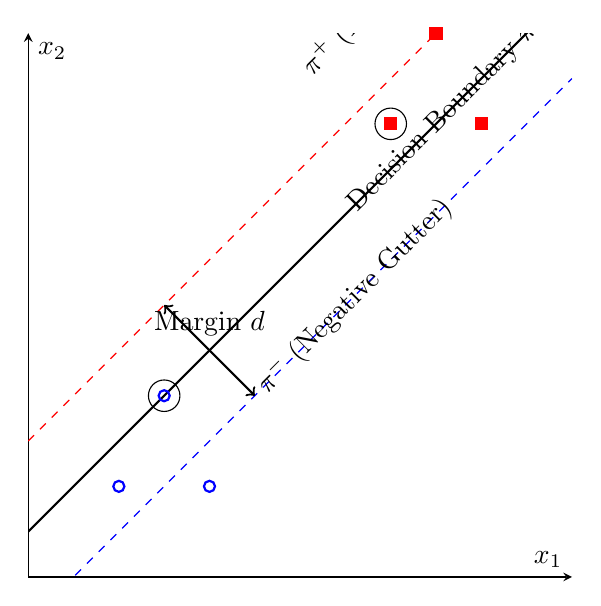
\begin{tikzpicture}
    \begin{axis}[
        xlabel={$x_1$}, ylabel={$x_2$},
        axis lines=middle,
        xmin=0, xmax=6, ymin=0, ymax=6,
        width=0.7\textwidth, height=0.7\textwidth,
        ticks=none
    ]
    % Data Points
    \addplot[only marks, mark=o, color=blue, thick] coordinates {(1,1) (2,1) (1.5,2)};
    \addplot[only marks, mark=square*, color=red, thick] coordinates {(4,5) (5,5) (4.5,6)};
    
    % Support Vectors (Circle them)
    \draw[black, thin] (axis cs:1.5,2) circle(0.2cm);
    \draw[black, thin] (axis cs:4,5) circle(0.2cm);
    
    % Hyperplane (Solid)
    \addplot[domain=0:6, color=black, thick] {x + 0.5};
    \node[right, rotate=45] at (axis cs:3.5, 4) {Decision Boundary $\pi$};
    
    % Margins (Dashed)
    \addplot[domain=0:6, color=blue, dashed] {x + 0.5 - 1.0}; % Shifted down
    \node[right, rotate=45] at (axis cs:2.5, 2) {$\pi^-$ (Negative Gutter)};
    
    \addplot[domain=0:6, color=red, dashed] {x + 0.5 + 1.0}; % Shifted up
    \node[right, rotate=45] at (axis cs:3, 5.5) {$\pi^+$ (Positive Gutter)};
    
    % Margin Arrow
    \draw[<->, thick] (axis cs:2.5, 2) -- (axis cs:1.5, 3);
    \node at (axis cs:2, 2.8) {Margin $d$};
    
    \end{axis}
\end{tikzpicture}
\caption{The Street (Margin). The algorithm pushes the dashed lines as far apart as possible until they hit the data points.}
\label{fig:svm_margin}
\end{figure}

\section{Core Terminology}
This geometry gives rise to three key definitions.

\begin{definition}
\textbf{Hyperplane ($\pi$)}: The decision boundary decision surface. In 2D, it is a line ($w^T x + b = 0$). Ideally, it lies exactly in the middle of the street.
\end{definition}

\begin{definition}
\textbf{Margin ($d$)}: The perpendicular distance between the two marginal planes (the "gutters"). SVM's goal is to \textbf{Maximize} this distance.
\end{definition}

\begin{definition}
\textbf{Support Vectors}: The specific data points that lie exactly on the edge of the margin. They "support" or "hold" the street in place.
\end{definition}

\textbf{Why is this called ``Support Vector Machine''?}
\\ Because the entire model is defined \textit{only} by these Support Vectors.
\\ If you delete the 99\% of data points that are far away from the road, the road does not move. The non-support vectors are mathematically irrelevant. This makes SVM distinct from Logistic Regression (which is affected by all points).

\section{Implementation in Python}
\begin{lstlisting}[language=Python, caption=Basic SVM Classifier]
from sklearn.svm import SVC
from sklearn.datasets import make_blobs
from sklearn.model_selection import train_test_split
from sklearn.preprocessing import StandardScaler

# Generate sample data
X, y = make_blobs(n_samples=100, centers=2, random_state=42)

# Scale features (important for SVM)
scaler = StandardScaler()
X_scaled = scaler.fit_transform(X)

# Train SVM
svm = SVC(kernel='linear', C=1.0)
svm.fit(X_scaled, y)

print(f"Number of Support Vectors: {len(svm.support_vectors_)}")
print(f"Accuracy: {svm.score(X_scaled, y):.2f}")
\end{lstlisting}

\section{HOTS: Interview Questions}
\textbf{Q1: Why is SVM called a ``Maximum Margin Classifier''?}
\begin{itemize}
    \item Because SVM explicitly tries to find the hyperplane that maximizes the distance (margin) between the decision boundary and the nearest data points (support vectors).
\end{itemize}

\textbf{Q2: How does SVM differ from Logistic Regression?}
\begin{itemize}
    \item Logistic Regression minimizes log-loss and is affected by all data points.
    \item SVM maximizes margin and is affected only by support vectors.
    \item SVM uses Hinge Loss, Logistic Regression uses Log Loss.
\end{itemize}

% ========================================
% SECTION: QUICK REFERENCE
% ========================================
\section{Quick Reference Card}

\begin{center}
\fbox{\parbox{0.9\textwidth}{
\textbf{SVM INTUITION - CHEAT SHEET}
\vspace{0.3cm}

\textbf{Core Idea}: Find the ``widest street'' (maximum margin) separating classes

\textbf{Key Components}:
\begin{itemize}
    \item \textbf{Hyperplane}: Decision boundary $w^Tx + b = 0$
    \item \textbf{Margin}: Distance between boundary and nearest points
    \item \textbf{Support Vectors}: Points on the margin edge (the VIPs)
\end{itemize}

\textbf{Margin Width}: $\frac{2}{||w||}$ (maximize by minimizing $||w||$)

\textbf{SVM vs Logistic Regression}:
\begin{center}
\begin{tabular}{|l|l|l|}
\hline
& \textbf{SVM} & \textbf{LogReg} \\ \hline
Loss & Hinge & Log \\ \hline
Points Used & Support Vectors only & All \\ \hline
Goal & Max Margin & Min Log-Loss \\ \hline
\end{tabular}
\end{center}

\textbf{Sklearn}: \texttt{SVC(kernel='linear', C=1.0)}

\textbf{Interview Gold}:
\begin{itemize}
    \item Only support vectors affect the decision
    \item MUST scale features (distance-based)
    \item C controls margin width vs errors tradeoff
\end{itemize}
}}

\chapter{The Mathematics of SVM}
\label{chap:svm_math}

% ========================================
% SECTION 1: DERIVING MARGIN WIDTH
% ========================================
\section{Deriving the Width of the Street}
How do we turn ``Maximize the Road'' into math?
We define our three planes:
\begin{enumerate}
    \item \textbf{Decision Boundary}: $w^T x + b = 0$
    \item \textbf{Positive Gutter}: $w^T x + b = +1$
    \item \textbf{Negative Gutter}: $w^T x + b = -1$
\end{enumerate}
(Why 1 and -1? It is just a scaling convention. We can always scale $w$ and $b$ to make this true for the nearest points.)

\subsection{Step-by-Step Margin Derivation}
\textbf{Goal}: Find the distance $d$ between the two parallel planes $w^T x + b = 1$ and $w^T x + b = -1$.

\textbf{Step 1}: Pick any point $x_1$ on the positive gutter: $w^T x_1 + b = 1$.

\textbf{Step 2}: The projection along the normal direction (which is $\frac{w}{||w||}$) to the negative gutter gives us: $x_2 = x_1 - d \cdot \frac{w}{||w||}$

\textbf{Step 3}: Since $x_2$ lies on the negative gutter: $w^T x_2 + b = -1$

\textbf{Step 4}: Substitute $x_2$:
\begin{align}
w^T \left( x_1 - d \cdot \frac{w}{||w||} \right) + b &= -1 \\
w^T x_1 + b - d \cdot \frac{w^T w}{||w||} &= -1 \\
1 - d \cdot \frac{||w||^2}{||w||} &= -1 \\
1 - d \cdot ||w|| &= -1 \\
d \cdot ||w|| &= 2
\end{align}

\textbf{Result}:
\begin{equation}
\boxed{d = \frac{2}{||w||}}
\end{equation}

% ========================================
% SECTION 2: HARD MARGIN OPTIMIZATION
% ========================================
\section{The Optimization Problem (Hard Margin)}
To get the widest street, we want to \textbf{Maximize $d$}.
\begin{itemize}
    \item $\text{Maximize } \frac{2}{||w||} \iff \text{Minimize } ||w||$.
    \item For calculus reasons (easier derivatives), minimizing $||w||$ is equivalent to minimizing $\frac{1}{2}||w||^2$.
\end{itemize}

\begin{definition}
\textbf{SVM Primal Problem (Hard Margin)}:
$$ \min_{w, b} \frac{1}{2} ||w||^2 $$
Subject to the constraint that every point $i$ is correctly classified \textit{outside} the gutter:
$$ y_i (w^T x_i + b) \ge 1 \quad \forall i $$
\end{definition}

% ========================================
% SECTION 3: SOFT MARGIN
% ========================================
\section{Soft Margin SVM (Handling Reality)}
Real-life data is messy. You might have one Red point deep inside the Blue cluster (Noise or Outlier).
If we insist on a ``Hard Margin'' (Perfect separation), the margin will become tiny or no solution will exist.

\subsection{Slack Variables ($\xi$)}
We allow the model to make some mistakes, but we penalize them. We introduce a \textbf{Slack Variable} $\xi_i$ (Greek: Zeta) for each point.

\begin{itemize}
    \item $\xi_i = 0$: Point is correctly classified and \textit{outside} the margin (Safe).
    \item $0 < \xi_i < 1$: Point is correct but \textit{inside} the margin (Margin Violation).
    \item $\xi_i \ge 1$: Point is \textbf{Misclassified} (On the wrong side of the hyperplane).
\end{itemize}

\begin{figure}[htbp]
\centering
\includegraphics[width=0.7\textwidth]{../02-supervised/assets/svm_slack_variables_concept.png}
\caption{Slack Variables: $\xi=0$ (safe), $0<\xi<1$ (margin violation), $\xi \ge 1$ (misclassified).}
\label{fig:slack_vars}
\end{figure}

\subsection{The Soft Margin Objective}
\begin{equation}
    J = \underbrace{\frac{1}{2}||w||^2}_{\text{Maximize Margin}} + C \underbrace{\sum_{i=1}^{n} \xi_i}_{\text{Minimize Errors}}
\end{equation}

% ========================================
% SECTION 4: THE C HYPERPARAMETER
% ========================================
\section{The Hyperparameter C}
$C$ controls the penalty for misclassification. It is the \textbf{boss} of the bias-variance trade-off.

\begin{itemize}
    \item \textbf{High C} (``I hate errors''):
    \begin{itemize}
        \item The model tries hard to classify everyone correctly.
        \item Result: Narrow margin, complex boundary.
        \item Risk: \textbf{Overfitting} (High Variance).
    \end{itemize}
    \item \textbf{Low C} (``I don't mind errors''):
    \begin{itemize}
        \item The model prioritizes a wider margin over perfect classification.
        \item Result: Wide margin, smooth boundary, ignores outliers.
        \item Risk: \textbf{Underfitting} (High Bias).
    \end{itemize}
\end{itemize}

\textbf{Analogy}: $C$ is like a ``Fine'' for parking illegally.
\begin{itemize}
    \item High $C$: Fine is \$1 Million. You will never park illegally (Hard Margin).
    \item Low $C$: Fine is \$1. You might park illegally if it's convenient (Soft Margin).
\end{itemize}

\begin{figure}[htbp]
\centering
\includegraphics[width=0.8\textwidth]{../02-supervised/assets/svm_c_parameter_comparison.png}
\caption{Effect of C: High C overfits to noise, Low C creates a robust boundary.}
\label{fig:c_param}
\end{figure}

% ========================================
% SECTION 5: HINGE LOSS
% ========================================
\section{Hinge Loss}
Modern SVM implementations (like Scikit-Learn's \texttt{SGDClassifier}) view this as a Loss Function minimization problem. The loss used is \textbf{Hinge Loss}.

\begin{definition}
\textbf{Hinge Loss}:
\begin{equation}
    L(y, f(x)) = \max(0, 1 - y \cdot f(x))
\end{equation}
Where $y \in \{-1, +1\}$ is the true label and $f(x) = w^T x + b$ is the raw prediction.
\end{definition}

\textbf{How it works}:
\begin{itemize}
    \item \textbf{Case 1: Correct and Safe} ($y \cdot f(x) \ge 1$):
    \begin{itemize}
        \item $1 - (\text{Large positive}) < 0$.
        \item $\max(0, \text{Negative}) = 0$. \textbf{No Loss}.
    \end{itemize}
    \item \textbf{Case 2: Correct but in Margin} ($0 < y \cdot f(x) < 1$):
    \begin{itemize}
        \item Loss is small positive.
    \end{itemize}
    \item \textbf{Case 3: Misclassified} ($y \cdot f(x) < 0$):
    \begin{itemize}
        \item Example: True $y = +1$, Predicted $f(x) = -2$. Product $= -2$.
        \item $1 - (-2) = 3$. Loss is \textbf{3} (Linear penalty).
    \end{itemize}
\end{itemize}

\begin{figure}[htbp]
\centering
\includegraphics[width=0.6\textwidth]{../02-supervised/assets/hinge_loss_graph.png}
\caption{Hinge Loss: Flat at 0 for correct predictions, then rises linearly.}
\label{fig:hinge_loss}
\end{figure}

% ========================================
% SECTION 6: C VS LAMBDA
% ========================================
\section{Connection to Regularization: C vs $\lambda$}
In Logistic Regression, we used Regularization ($\lambda$) to \textit{prevent} overfitting:
$$ \text{Cost} = \text{Log Loss} + \lambda ||w||^2 $$
High $\lambda$: Huge penalty on weights $\to$ Simple Model (Underfitting).

In SVM, we use $C$ to \textit{penalize} errors:
$$ \text{Cost} = C \times \text{Hinge Loss} + \frac{1}{2}||w||^2 $$
High $C$: Huge penalty on errors $\to$ Complex Model (Overfitting).

\begin{definition}
\textbf{Key Relationship}: $C$ is inversely proportional to $\lambda$.
$$ C \propto \frac{1}{\lambda} $$
\begin{itemize}
    \item \textbf{Large C} $\approx$ \textbf{Small $\lambda$} (Weak Regularization, High Variance).
    \item \textbf{Small C} $\approx$ \textbf{Large $\lambda$} (Strong Regularization, High Bias).
\end{itemize}
\end{definition}

% ========================================
% SECTION 7: HOTS QUESTIONS
% ========================================
\section{HOTS: Interview Questions}
\textbf{Q1: What is the role of Slack Variables in SVM?}
\begin{itemize}
    \item They allow the SVM to tolerate some misclassifications in exchange for a wider margin.
    \item $\xi_i$ measures how much point $i$ violates the margin constraint.
\end{itemize}

\textbf{Q2: How do you choose the hyperparameter C?}
\begin{itemize}
    \item Use cross-validation (\texttt{GridSearchCV}).
    \item Try a logarithmic range: $C \in [0.001, 0.01, 0.1, 1, 10, 100]$.
\end{itemize}

\textbf{Q3: Why is Hinge Loss preferred over Log Loss for SVM?}
\begin{itemize}
    \item Hinge Loss only penalizes points that are misclassified or within the margin.
    \item Log Loss penalizes all points, even those far from the boundary.
    \item Hinge Loss leads to sparse solutions (only support vectors matter).
\end{itemize}

\chapter{Kernels and Non-Linear SVM}
\label{chap:svm_kernels}

\section{The Limits of Linearity}
Everything we discussed so far assumes the data is \textbf{Linearly Separable}.
But what if the data looks like a target board? (Red points in the bullseye, Blue points in the outer ring).
No straight line can separate these.

\section{The Kernel Trick}
SVM has a superpower. If we can't separate data in 2D, we can project it into 3D (or higher) where it \textit{might} be separable.

\begin{definition}
\textbf{The Kernel Trick}: A technique that maps input vectors into a higher-dimensional feature space without explicitly computing the coordinates in that space. It allows valid linear separation in high dimensions that corresponds to non-linear separation in the original space.
\end{definition}

\subsection{Example: 1D to 2D}
Imagine points on a line:
\begin{itemize}
    \item Red points at $x = -1, 0, 1$ (Center).
    \item Blue points at $x = -5, 5$ (Edges).
\end{itemize}
We cannot separate them with a single point (cut).
\\ \textbf{Transformation}: Let $y = x^2$.
\begin{itemize}
    \item Red points become $(0,0), (-1,1), (1,1)$. Height is low.
    \item Blue points become $(-5, 25), (5, 25)$. Height is high.
\end{itemize}
Now, we can draw a horizontal line at $y=10$. Everything below is Red, everything above is Blue.
In the original 1D space, this translates to \textit{two} cuts at $-3$ and $+3$.

\begin{figure}[htbp]
\centering
\begin{tikzpicture}
    % 1D Space (Bottom)
    \draw[->] (-4, -1) -- (4, -1) node[right] {$x$};
    \foreach \x/\c in {-1/red, 0/red, 1/red, -3.5/blue, 3.5/blue}
        \fill[\c] (\x, -1) circle (3pt);
    \node at (0, -1.5) {1D: Not Separable};
    
    % Projection Arrows
    \draw[->, dashed, orange] (-3.5, -0.8) -- (-3.5, 3.5^2/4 - 1);
    \draw[->, dashed, orange] (0, -0.8) -- (0, 0 - 1);
    
    % 2D Space (Parabola)
    \begin{axis}[
        at={(0,0)},
        width=0.6\textwidth, height=0.5\textwidth,
        axis lines=middle,
        ymin=-1, ymax=15,
        ticks=none,
        xlabel=$x$, ylabel=$x^2$
    ]
    % Parabola Curve
    \addplot[domain=-4:4, smooth, black] {x^2};
    
    % Points
    \addplot[only marks, mark=*, color=red] coordinates {(0,0) (-1,1) (1,1)};
    \addplot[only marks, mark=*, color=blue] coordinates {(-3.5, 12.25) (3.5, 12.25)};
    
    % Separator
    \addplot[domain=-4:4, dashed, green!50!black, thick] {6};
    \node[right, color=green!50!black] at (axis cs:2, 6.5) {Linear Separator};
    \end{axis}
\end{tikzpicture}
\caption{Kernel Trick: Points non-separable in 1D become separable when projected to $y=x^2$.}
\label{fig:kernel_trick}
\end{figure}

\section{Popular Kernels}
\subsection{1. Polynomial Kernel}
Maps data to polynomial combinations (like $x_1^2, x_1x_2, x_2^2$).
$$ K(x, y) = (x^T y + c)^d $$
Good for simple curved boundaries.

\subsection{2. RBF (Radial Basis Function) Kernel}
This is the default and most powerful kernel. It behaves like a \textbf{Similarity Function}.
\begin{equation}
    K(x, y) = \exp(-\gamma ||x - y||^2)
\end{equation}
It essentially lifts the support vectors into infinite dimensions, creating "mountains" (Gaussian bells) around the data points.

\section{Understanding Gamma ($\gamma$)}
The RBF kernel has a critical hyperparameter: **Gamma**.
$$ \gamma = \frac{1}{2 \sigma^2} $$
\begin{itemize}
    \item \textbf{Low Gamma}: Wide Gaussian Bell. A single point influences a huge area. The decision boundary is smooth.
    \item \textbf{High Gamma}: Narrow, pointy Gaussian Bell. A point only influences its immediate neighborhood. This leads to ``Islands'' around points. \textbf{Overfitting}.
\end{itemize}

\section{Implementation in Python}
\begin{lstlisting}[language=Python, caption=SVM with RBF Kernel]
from sklearn.svm import SVC
from sklearn.datasets import make_circles
from sklearn.model_selection import train_test_split
from sklearn.preprocessing import StandardScaler

# Non-linearly separable data (concentric circles)
X, y = make_circles(n_samples=200, noise=0.1, factor=0.3)

# Scale features
scaler = StandardScaler()
X_scaled = scaler.fit_transform(X)

# Train SVM with RBF kernel
svm_rbf = SVC(kernel='rbf', C=1.0, gamma='scale')
svm_rbf.fit(X_scaled, y)

print(f"Accuracy: {svm_rbf.score(X_scaled, y):.2f}")
\end{lstlisting}

\section{HOTS: Interview Questions}
\textbf{Q1: What is the Kernel Trick and why is it useful?}
\begin{itemize}
    \item The Kernel Trick allows SVM to work in a high-dimensional feature space without explicitly computing the coordinates, using only dot products. This makes non-linear separation computationally feasible.
\end{itemize}

\textbf{Q2: How do you choose between Polynomial and RBF kernels?}
\begin{itemize}
    \item RBF is the default choice and works well in most cases.
    \item Polynomial is useful when you know the data has a polynomial relationship.
    \item Use cross-validation to compare performance.
\end{itemize}

%\chapter{Support Vector Machines (SVM)}

\section{Introduction}
Support Vector Machines (SVM) take a geometric approach to classification. Unlike Logistic Regression which finds \textit{any} separating line, SVM aims to find the \textbf{Best} separating line.

\subsection{Geometric Intuition: The Widest Street}
Imagine the decision boundary as a road.
\begin{itemize}
    \item We want the road (\textbf{Margin}) to be as wide as possible without touching any data points.
    \item A wider margin implies the model is more confident and robust to outliers.
\end{itemize}

\subsection{Terminology}
\begin{itemize}
    \item \textbf{Hyperplane ($\pi$)}: The central decision boundary ($w^T x + b = 0$).
    \item \textbf{Support Vectors}: The specific data points that lie on the edge of the margin. The entire model depends \textit{only} on these points.
    \item \textbf{Margin ($d$)}: The distance between the positive and negative class boundaries.
\end{itemize}

\section{Mathematical Formulation}

\subsection{Hard Margin (Perfect Separation)}
Assuming the data is perfectly separable, we want to maximize the margin $d$.
It can be derived that the margin width is $d = \frac{2}{||w||}$.
To maximize $d$, we must \textbf{minimize $||w||$} (or effectively $\frac{1}{2}||w||^2$).

\textbf{Optimization Goal:}
\begin{equation}
    \min_{w,b} \frac{1}{2} ||w||^2
\end{equation}
\textbf{Subject to constraint:}
\begin{equation}
    y_i (w^T x_i + b) \ge 1 \quad \forall i
\end{equation}
This ensures that every point is correctly classified and lies outside the margin.

\subsection{Soft Margin (Handling Outliers)}
Real-world data is rarely perfectly separable. We introduce \textbf{Slack Variables ($\xi_i$)} to allow some points to violate the margin.

\textbf{New Objective:}
\begin{equation}
    \min_{w,b} \left[ \frac{1}{2} ||w||^2 + C \sum_{i=1}^{n} \xi_i \right]
\end{equation}

\subsubsection{The Hyperparameter C}
$C$ controls the trade-off:
\begin{itemize}
    \item \textbf{High C}: Strict penalty for errors. Tries to classify everything correctly. Risk of \textbf{Overfitting}.
    \item \textbf{Low C}: Loose penalty. Allows wider margin even if some points are misclassified. Risk of \textbf{Underfitting} (but more robust).
\end{itemize}

\section{Kernels and Non-Linearity}
What if the data is not linearly separable (e.g., concentric circles)?
We use the \textbf{Kernel Trick} to map data into a higher-dimensional space where it becomes linearly separable.

\subsection{Common Kernels}
\begin{itemize}
    \item \textbf{Polynomial Kernel}: Maps to polynomial dimensions ($x^2, x^3$).
    \item \textbf{RBF (Radial Basis Function) Kernel}: Maps to infinite dimensions. Creates "hills" around points.
        \begin{equation}
            K(x_1, x_2) = \exp(-\gamma ||x_1 - x_2||^2)
        \end{equation}
\end{itemize}

\subsection{The Gamma ($\gamma$) Parameter}
For RBF Kernel:
\begin{itemize}
    \item \textbf{High Gamma}: Each point has narrow influence. Creates complex, wiggly boundaries. (Overfitting).
    \item \textbf{Low Gamma}: Points have wide influence. Creates smooth boundaries. (Underfitting).
\end{itemize}

\section{Implementation in Python}
\textbf{CRITICAL}: SVM is distance-based, so \textbf{Feature Scaling} is mandatory.

\begin{lstlisting}[language=Python, caption=SVM Implementation with Scaling]
from sklearn.svm import SVC
from sklearn.preprocessing import StandardScaler
from sklearn.model_selection import train_test_split
from sklearn.datasets import load_breast_cancer

# 1. Load Data
data = load_breast_cancer()
X, y = data.data, data.target
X_train, X_test, y_train, y_test = train_test_split(X, y, test_size=0.2)

# 2. Scale Data (Mandatory)
scaler = StandardScaler()
X_train_scaled = scaler.fit_transform(X_train)
X_test_scaled = scaler.transform(X_test)

# 3. Train Model
# Kernel='rbf' is default.
model = SVC(kernel='rbf', C=1.0, gamma='scale')
model.fit(X_train_scaled, y_train)

# 4. Evaluate
print("Accuracy:", model.score(X_test_scaled, y_test))
\end{lstlisting}
 % Refactored

\part{K-Nearest Neighbors}
\chapter{K-Nearest Neighbors (KNN)}
\label{chap:knn_intuition}

\section{The Core Philosophy}
\begin{quote}
``You are the average of the five people you spend the most time with.'' -- Jim Rohn
\end{quote}
This self-help quote is the exact mathematical foundation of the K-Nearest Neighbors algorithm.
The assumption is simple: \textbf{Similar things exist in close proximity}.

\begin{definition}
\textbf{K-Nearest Neighbors (KNN)}: A non-parametric supervised learning algorithm that classifies a new data point based on the majority class of its 'K' closest neighbors in the feature space.
\end{definition}

\section{How the Algorithm Works}
KNN is deceptively simple. It follows three steps:
\begin{enumerate}
    \item \textbf{Store}: Save the training data. (That's it. No math yet).
    \item \textbf{Distance}: When a new point $X_{new}$ arrives, calculate its distance to every single point in the database.
    \item \textbf{Vote}: Pick the top $K$ closest points. Let them vote. The majority wins.
\end{enumerate}

\begin{figure}[htbp]
\centering
\includegraphics[width=0.7\textwidth]{../02-supervised/assets/knn_intuition_concept.png}
\caption{KNN finds the K nearest neighbors and lets them vote on the new point's class.}
\label{fig:knn_intuition}
\end{figure}

\section{Lazy vs Eager Learning}
This highlights a fundamental distinction in ML.

\begin{definition}
\textbf{Eager Learners} (e.g., Linear Regression, SVM): They analyze the training data \textit{beforehand} and construct a generalized model formula (weights $w$ and bias $b$). Once trained, they can discard the original data. Prediction is fast ($O(1)$).
\end{definition}

\begin{definition}
\textbf{Lazy Learners} (e.g., KNN): They do not build a model during training. They strictly memorize the data. All the computation happens during Prediction time. Prediction is slow ($O(N)$).
\end{definition}

\section{Regression with KNN}
KNN is not limited to Classification.
If we want to predict a continuous value (e.g., House Price):
\begin{itemize}
    \item Instead of a Majority Vote (Mode), we calculate the \textbf{Average (Mean)} of the neighbors.
    \item If the 3 nearest houses cost \$100k, \$120k, and \$110k, the prediction is \$110k.
\end{itemize}

\section{Implementation in Python}
\begin{lstlisting}[language=Python, caption=KNN Classifier]
from sklearn.neighbors import KNeighborsClassifier
from sklearn.datasets import load_iris
from sklearn.model_selection import train_test_split
from sklearn.preprocessing import StandardScaler

# Load data
X, y = load_iris(return_X_y=True)
X_train, X_test, y_train, y_test = train_test_split(X, y, test_size=0.2)

# Scale features (CRITICAL for KNN!)
scaler = StandardScaler()
X_train_s = scaler.fit_transform(X_train)
X_test_s = scaler.transform(X_test)

# Train KNN
knn = KNeighborsClassifier(n_neighbors=5)
knn.fit(X_train_s, y_train)

print(f"Accuracy: {knn.score(X_test_s, y_test):.2f}")
\end{lstlisting}

\section{HOTS: Interview Questions}
\textbf{Q1: Why is KNN called a ``Lazy Learner''?}
\begin{itemize}
    \item Because it does no work during training. It simply stores the data. All computation (distance calculation) happens at prediction time.
\end{itemize}

\textbf{Q2: What are the main disadvantages of KNN?}
\begin{itemize}
    \item Slow prediction time ($O(N \cdot D)$ where N = samples, D = dimensions).
    \item Requires feature scaling.
    \item Suffers from the Curse of Dimensionality.
    \item Sensitive to noisy data and outliers.
\end{itemize}

% ========================================
% SECTION: QUICK REFERENCE
% ========================================
\section{Quick Reference Card}

\begin{center}
\fbox{\parbox{0.9\textwidth}{
\textbf{K-NEAREST NEIGHBORS - CHEAT SHEET}
\vspace{0.3cm}

\textbf{Algorithm}:
\begin{enumerate}
    \item Store training data (no work!)
    \item For new point: compute distance to all stored points
    \item Pick K nearest neighbors, majority vote
\end{enumerate}

\textbf{Distance Metrics}:
\begin{itemize}
    \item Euclidean: $\sqrt{\sum(x_i - y_i)^2}$ (default)
    \item Manhattan: $\sum|x_i - y_i|$
\end{itemize}

\textbf{Choosing K}:
\begin{itemize}
    \item Use odd K for binary classification (avoid ties)
    \item Use Elbow Method or Cross-Validation
\end{itemize}

\textbf{Sklearn}: \texttt{KNeighborsClassifier(n\_neighbors=5)}

\textbf{Interview Gold}:
\begin{itemize}
    \item Lazy Learner: no training, all work at prediction
    \item MUST scale features (distance-based)
    \item Curse of Dimensionality: fails in high-D
\end{itemize}
}}

\chapter{Distance Metrics and Hyperparameters}
\label{chap:knn_metrics}

\section{Defining "Nearness"}
To say two points are "close", we need a ruler. In math, this ruler is the \textbf{Distance Metric}.

\subsection{1. Euclidean Distance (L2 Norm)}
This is the straight-line distance, derived from the Pythagorean theorem. It is the default for most continuous data.
\begin{definition}
$$ d(p, q) = \sqrt{ \sum_{i=1}^{n} (p_i - q_i)^2 } $$
\end{definition}

\subsection{2. Manhattan Distance (L1 Norm)}
Also known as "Taxicab Geometry". Imagine a grid-like city (Manhattan). You cannot walk through buildings (diagonal); you must walk along the streets.
\begin{definition}
$$ d(p, q) = \sum_{i=1}^{n} | p_i - q_i | $$
\end{definition}
This is often better for high-dimensional sparse data.

\section{The Cardinal Sin: Forgetting to Scale}
KNN is strictly based on distance magnitude. This makes it dangerously sensitive to the scale of input features.

\textbf{Example Failure}:
Imagine two features:
\begin{itemize}
    \item \textbf{Age}: 20 to 80 (Range = 60).
    \item \textbf{Salary}: 20,000 to 100,000 (Range = 80,000).
\end{itemize}
If we compute Euclidean Distance:
$$ \sqrt{(Age_1-Age_2)^2 + (Salary_1-Salary_2)^2} $$
The term $(Salary)^2$ will result in billions. The term $(Age)^2$ will be tiny.
The distance will be 99.99\% determined by Salary. The algorithm effectively \textbf{ignores Age}.

\begin{quote}
\textbf{Rule}: You must always apply \textbf{StandardScaler} (normalize to Mean=0, Variance=1) before running KNN.
\end{quote}

\section{The Hyperparameter K}
\begin{itemize}
    \item \textbf{Small K (e.g., K=1)}: The model looks at only the single nearest person. If that person is an outlier (noise), the prediction is wrong. \textbf{High Variance (Overfitting)}.
    \item \textbf{Large K (e.g., K=100)}: The model averages over a huge crowd. It loses local detail and tends to predict the majority class for everyone. \textbf{High Bias (Underfitting)}.
\end{itemize}

\chapter{The Curse of Dimensionality}
\label{chap:knn_curse}

\section{Why KNN Fails in High Dimensions}
Human intuition works well in 2D and 3D. But data often has hundreds of dimensions (features).
As dimensions increase, we encounter a paradox known as the \textbf{Curse of Dimensionality}.

\section{The Sparsity Problem}
Imagine a unit cube (side length 1).
\begin{itemize}
    \item **1D**: 10 points cover the line well.
    \item **2D**: To cover a square with same density, you need $10^2 = 100$ points.
    \item **3D**: You need $10^3 = 1000$ points.
    \item **100D**: You need $10^{100}$ points.
\end{itemize}
In high dimensions, unless you have infinite data, the space is mostly \textbf{Empty Air}.
Points are so far apart that "Nearest Neighbor" implies "Least Far Neighbor". They aren't actually close.

\section{Weighted KNN (Distance Weighting)}
A standard KNN uses a simple generic vote: "3 neighbors say Red, 2 say Blue $\rightarrow$ Red wins".
But what if the 3 Red neighbors are very far away, and the 2 Blue neighbors are extremely close?

We can fix this by **Weighting** the vote.
\begin{definition}
\textbf{Distance Weighting}: The influence of a neighbor's vote is proportional to the inverse of its distance.
$$ \text{Weight} = \frac{1}{\text{distance}^2} $$
\end{definition}
This ensures that local points matter more than distant points, helping with both outliers and imbalanced data.

\section{HOTS Questions}
\textbf{Q1: Why does KNN fail with raw Image pixels?}
\\ \textit{Answer}: A 28x28 image has 784 dimensions. In 784D space, all images are far apart (Curse of Dimensionality). Euclidean distance between two images is often meaningless (shifting an image by 1 pixel changes all pixel values but the image is the same). Convolutional Neural Networks (CNNs) are needed to extract lower-dimensional features first.

%\chapter{K-Nearest Neighbors (KNN)}

\section{Introduction}
\begin{quote}
    ``You are the average of the five people you spend the most time with.'' — Jim Rohn
\end{quote}
This quote perfectly summarizes KNN. It is a simple, intuitive algorithm that classifies a new data point based on the majority class of its neighbors.

\subsection{Standard vs Lazy Learners}
\begin{itemize}
    \item \textbf{Eager Learners (Linear Regression, SVM, Trees)}: try to learn a function $f(x)$ during training. They discard the training data after building the model.
    \item \textbf{Lazy Learners (KNN)}: do \textbf{zero work} during training. They simply memorize the dataset. All computation (distance calculation) happens at \textbf{Inference Time}.
\end{itemize}

\section{The Algorithm}
For a new point $p$:
\begin{enumerate}
    \item \textbf{Calculate Distance}: Compute distance between $p$ and every training point.
    \item \textbf{Sort}: Find the $K$ points with the smallest distances.
    \item \textbf{Vote}:
    \begin{itemize}
        \item \textbf{Classification}: Return the Mode (Majority Class).
        \item \textbf{Regression}: Return the Mean (Average Value).
    \end{itemize}
\end{enumerate}

\subsection{Distance Metrics}
\begin{itemize}
    \item \textbf{Euclidean Distance (L2)}: Straight line distance. (Standard).
    $$ d(x, y) = \sqrt{\sum (x_i - y_i)^2} $$
    \item \textbf{Manhattan Distance (L1)}: Grid-like distance.
    $$ d(x, y) = \sum |x_i - y_i| $$
\end{itemize}

\section{Choosing K (Bias-Variance Tradeoff)}
The value of $K$ is the most critical hyperparameter.
\begin{itemize}
    \item \textbf{Low K (e.g., K=1)}: Model is very complex and jagged. It captures noise. \textbf{High Variance (Overfitting)}.
    \item \textbf{High K}: Model becomes too smooth. It predicts the majority class everywhere. \textbf{High Bias (Underfitting)}.
    \item \textbf{Optimal K}: Found using Cross-Validation (Elbow Method). A common heuristic is $K = \sqrt{N}$.
\end{itemize}

\section{Curse of Dimensionality}
KNN fails when the number of features ($d$) is large.
In high-dimensional space, points become sparse, and the concept of "distance" loses meaning (all points are roughly equidistant). KNN requires dimensionality reduction (like PCA) for high-dimensional data.

\section{Implementation in Python}
\textbf{CRITICAL}: Because KNN uses distance, features with larger scales will dominate. You \textbf{MUST} use \texttt{StandardScaler}.

\begin{lstlisting}[language=Python, caption=KNN Implementation with Tuning]
import matplotlib.pyplot as plt
from sklearn.neighbors import KNeighborsClassifier
from sklearn.preprocessing import StandardScaler
from sklearn.model_selection import train_test_split, cross_val_score
from sklearn.datasets import load_breast_cancer

# 1. Load & Scale (MANDATORY)
data = load_breast_cancer()
scaler = StandardScaler()
X_scaled = scaler.fit_transform(data.data)
y = data.target

X_train, X_test, y_train, y_test = train_test_split(X_scaled, y, test_size=0.2)

# 2. Find Optimal K using Cross-Validation
k_values = range(1, 30, 2) # Odd numbers to avoid ties
cv_scores = []

for k in k_values:
    knn = KNeighborsClassifier(n_neighbors=k)
    scores = cross_val_score(knn, X_train, y_train, cv=10, scoring='accuracy')
    cv_scores.append(scores.mean())

# Plot Elbow Curve
plt.plot(k_values, cv_scores, marker='o')
plt.title('Accuracy vs K')
plt.show()

# 3. Train Final Model
best_k = 9 # Assume we found 9 is best
knn_final = KNeighborsClassifier(n_neighbors=best_k)
knn_final.fit(X_train, y_train)
print("Test Acc:", knn_final.score(X_test, y_test))
\end{lstlisting}
 % Refactored

\appendix
%\chapter{Data Preprocessing}
\label{chap:preprocessing}

Real-world data is messy. It has missing values, text instead of numbers, and different scales. Before we train any model, we must clean and prepare the data.

% ========================================
% SECTION 1: HANDLING MISSING VALUES
% ========================================
\section{Handling Missing Values}
Use \texttt{SimpleImputer} to fill in gaps.
\begin{itemize}
    \item \textbf{Numerical Data}: Replace with \texttt{mean} or \texttt{median}.
    \item \textbf{Categorical Data}: Replace with \texttt{most\_frequent} (mode) or a constant value like ``Unknown''.
\end{itemize}

\begin{lstlisting}[language=Python, caption=Handling Missing Values]
from sklearn.impute import SimpleImputer
import numpy as np

# Data with missing values (NaN)
X = np.array([[1, 2], [np.nan, 3], [7, 6]])

# Impute with Mean
imputer = SimpleImputer(strategy='mean')
X_clean = imputer.fit_transform(X)
# Result: NaN is replaced by (1+7)/2 = 4
\end{lstlisting}

% ========================================
% SECTION 2: CATEGORICAL DATA (ONE-HOT CODING)
% ========================================
\section{Handling Categorical Data}
Machine Learning models (like Linear Regression, SVM) only understand numbers. They cannot understand "Red", "Green", "Blue".

\subsection{Why NOT Label Encoding?}
If we assign Red=1, Green=2, Blue=3:
\begin{itemize}
    \item The model thinks Blue $>$ Green $>$ Red.
    \item It assumes an order (Ordinality) where none exists.
    \item Equation: $y = 3w$ (Blue) vs $y = 1w$ (Red). This is wrong.
\end{itemize}

\subsection{The Solution: One-Hot Encoding}
We create a new binary column for each category.
\begin{table}[htbp]
\centering
\begin{tabular}{|l|c|c|c|}
\hline
\textbf{Color} & \textbf{Is\_Red} & \textbf{Is\_Green} & \textbf{Is\_Blue} \\ \hline
Red & 1 & 0 & 0 \\ \hline
Green & 0 & 1 & 0 \\ \hline
Blue & 0 & 0 & 1 \\ \hline
\end{tabular}
\end{table}

\begin{lstlisting}[language=Python, caption=One-Hot Encoding]
from sklearn.preprocessing import OneHotEncoder
import pandas as pd

df = pd.DataFrame({'Color': ['Red', 'Green', 'Blue', 'Red']})

# Option 1: Pandas (Quick)
df_ohe = pd.get_dummies(df, columns=['Color'])

# Option 2: Scikit-Learn (Pipeline friendly)
encoder = OneHotEncoder(sparse=False, handle_unknown='ignore')
encoded_matrix = encoder.fit_transform(df[['Color']])
\end{lstlisting}

% ========================================
% SECTION 3: THE PREPROCESSING PIPELINE
% ========================================
\section{Putting It All Together: A Pipeline}
In production, we chain these steps using \texttt{Pipeline} and \texttt{ColumnTransformer}.

\begin{lstlisting}[language=Python, caption=Full Preprocessing Pipeline]
from sklearn.compose import ColumnTransformer
from sklearn.pipeline import Pipeline
from sklearn.preprocessing import StandardScaler, OneHotEncoder

# Define features
numeric_features = ['age', 'salary']
categorical_features = ['city', 'gender']

# 1. Pipe for Numbers: Impute -> Scale
num_pipe = Pipeline([
    ('imputer', SimpleImputer(strategy='median')),
    ('scaler', StandardScaler())
])

# 2. Pipe for Categories: Impute -> OneHot
cat_pipe = Pipeline([
    ('imputer', SimpleImputer(strategy='constant', fill_value='missing')),
    ('onehot', OneHotEncoder(handle_unknown='ignore'))
])

# 3. Combine
preprocessor = ColumnTransformer([
    ('num', num_pipe, numeric_features),
    ('cat', cat_pipe, categorical_features)
])

# 4. Final Model
model = Pipeline([
    ('preprocessor', preprocessor),
    ('classifier', LogisticRegression())
])
\end{lstlisting}


\end{document}
\sum_{i=1}^n x_i \equiv x_1 + x_2 +\cdots + x_n
\end{equation}


\end{document}